

\chapter{Positivity Preservation}
\label{cha:pos}

\section{Positive Solutions to ODEs}

\subsection{Motivation}

There are many problems which motivate the need for numerical methods which preserve positivity of the solution.
For example, consider the problem of simulating a chemical reaction.
We start with a finite amout of positive-valued species at the initial stage, and apply some numerical method to produce a result.
Despite being able to apply methods which have high orders of accuracy, traditional methods will not preserve positivity unconditionally.
If our numerical solution indicates that the concentrations of any number of species become negative, then our solution is not qualitatively accurate to a ``true'' solution.

Consider a problem given by $\dot{x} = f(x)$, with the initial condition $x(0) = x_0$.
For a one-dimensional problem, the true solution is positive if, given $x_0 \ge 0$, we have that $x(t) \ge 0$ for $t>0$.
Positivity of the numerical solution can be expressed as the condition that if $x_i \ge 0$ then $x_{i+1} \ge 0$ for all $i = 1, \mathellipsis, N$ timesteps in the computation.
Like always, $x$ may be vector-valued. If $x \in \mathds{R}^d$,
then the condition for positivity of the numerical solution applies element-wise to each component $x_i^{(k)}$ for $k = 1, \mathellipsis, d$.
Importantly, entries \textit{can} be zero. 

Methods which preserve positivity are a current area of research. It is difficult to produce numerical methods which both preserve positivity and maintain high order accuracy.
Moreover, it is very difficult to formulate positivity preserving methods for general problems.
Our approach will be to consider particular cases, where we can reduce the problem $\dot{x} = f(x)$ to a particular form,
and formulate positivity-preserving methods which are effective for these problems.

\subsection{The Graph-Laplacian Matrix}

\begin{figure}
    \centering
    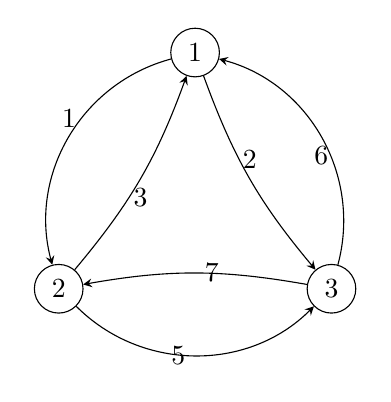
\begin{tikzpicture}[>=stealth, node distance=2cm]
        % Define vertices
        \node[circle, draw] (1) at (90:2cm) {1};
        \node[circle, draw] (2) at (210:2cm) {2};
        \node[circle, draw] (3) at (330:2cm) {3};
        
        % Draw edges
        \draw[->] (1) to [bend right=45] node[midway, above] {$1$} (2);
        \draw[->] (2) to [bend right=45] node[midway, left] {$5$} (3);
        \draw[->] (3) to [bend right=45] node[midway, below] {$6$} (1);
        
        \draw[->] (2) to [bend right=10] node[midway, below] {$3$} (1);
        \draw[->] (3) to [bend right=10] node[midway, right] {$7$} (2);
        \draw[->] (1) to [bend right=10] node[midway, above] {$2$} (3);
        % Thank you ChatGPT
    \end{tikzpicture}
    \caption{
    	A directed graph, given for the demonstration of a graph-Laplacian matrix, taken from Wikipedia \cite{Wikipedia_2024}.
    	Nodes are indexed from $1$ to $3$ and each directed edge has a given weight.
    	Each node is connected to the other.
    }
    \label{fig:graph1998}
\end{figure}

Before looking at positivity-preserving methods, we will consider problems which themselves must admit positivity-preserving solutions.
The notion of the graph-Laplacian matrix and the methods centered around it are taken from \cite{blanes_pos_2022}.

Our main focus will be on problems that we can write in the form 
\begin{equation*}
    \dot{x} = A(x)x
\end{equation*}
where $A$ is a graph-Laplacian matrix \cite{blanes_pos_2022}.

\begin{definition}
    A graph-Laplacian matrix $A \in \mathds{R}^{d \times d}$ is a square matrix that satisfies
    \begin{itemize}
        \item $\mathbf{1}^\intercal A = \mathbf{0}^\intercal ~~ \text{(its column sums are zero)}.$
        \item For all $i, j = 1, \mathellipsis, d$ where $i \ne j$ we have $A_{ij} \ge 0$.
        \item For all $i = 1, \mathellipsis, d$ we have $A_{ii} \le 0$
    \end{itemize}
\end{definition}

Note that here, $A$ can depend on $x$. The entries in $A(x)$ can contain entries of $x$ in any fashion, as long as the definition is satisfied.

The name ``graph-Laplacian'' comes from graph theory, and the definition is not universally agreed upon.
For our needs, we consider a graph-Laplacian matrix for a directional graph to be the in-degree matrix (empty diagonal) minus the in-degree adjacency matrix (diagonal) of the graph.
Consider the graph given by Figure \ref{fig:graph1998}.
The in-degree matrix $D$ for this graph is
\begin{equation*}
    D = \begin{bmatrix}
        9 & 0 & 0 \\
        0 & 8 & 0 \\
        0 & 0 & 7
    \end{bmatrix}
\end{equation*}
where $d_{ii}$ is the in-degree of vertex $i$ and $d_{ij}=0$ for $i \neq j$. 
The adjacency matrix $C$ is
\begin{equation*}
    C = \begin{bmatrix}
        0 & 1 & 2 \\
        3 & 0 & 5 \\
        6 & 7 & 0
    \end{bmatrix}
\end{equation*}
where $c_{ij}$ is the weight of the edge from vertex $i$ to vertex $j$.
We define the Laplacian matrix $A$ for a graph by
\begin{equation}
    A = C - D.
\end{equation}
We have covered this case for integers, however in general we will consider graph-Laplacian matrices over real numbers.
If a problem admits the reduction to graph-Laplacian form like the above,
we can show that the solution retains positivity.

\begin{theorem}[Preservation of Positivity \cite{blanes_pos_2022}]
    \label{thm:posgl}
    Solutions of $\dot{x} = A(x)x$ retain positivity if $A$ is graph-Laplacian.
\end{theorem}
\begin{proof}
    Consider the solution $x(t^*)$ at time $t^*$. Assume that there are indices $k \in \{1,\mathellipsis, d\}$ where all entries $x_k(t^*)$ are zero and the rest are strictly positive.
    Then the $k$-th equation in the matrix system is
    \begin{equation*}
        \dot{x}_k(t^*) = \sum_{l = 1}^{d} A_{kl}(x(t^*))x_l(t^*).
    \end{equation*}
    Entry $A_{kk}$ is negative, but we assumed $x_k(t^*)=0$ so the only contributions to the sum are the $A_{kl}$ and $x_l$ for $l \ne k$.
    Some of the $x_l$ may be zero but all the rest are positive, so we have $\dot{x}_k \ge 0$.
    Note that equality is attained if all the $x_k$ are zero which is the trivial solution. 
    Assume instead that every entry $x_k(t^*)$ is non-zero and hence positive.
    In this case there are no restrictions on the derivative of the $k$-th entry - the $A_{kk}$ term means this derivative can be negative.
    The $x_k$ term can go to zero, but since the derivative is strictly non-negative at zero, we will retain positivity.
\end{proof}

We have shown that the graph-Laplacian form is a suitable structure for problems where we are concerned about positivity preservation.
From now on, for a vector solution $x \in \mathds{R}^d$ we will write $x \ge 0$ to mean that each element $x_k \ge 0$ for $k = 1, \mathellipsis, d$.
Before moving on to numerical methods that preserve positivity of these problems, we will consider a few points of note.

\subsection{Non-autonomous Systems}

Our analysis so far has focused on problems $\dot{x} = A(x)x$, which are autonomous.
Examples in positivity preservation can often be non-autonomous, which we would write as $\dot{x} = A(x,t)x$.
The particular details of problems involving the graph-Laplacian matrix can be easily analogised to the non-autonomous case.
As such, we will usually only consider problems in the autonomous form, unless it is necessary to the analysis.

Some problems can involve several different timescales,
in which case time-dependence is very important to account for.

\subsection{Conservation of Mass}

%% how graph laplacians also maintain conservation of mass and why this is nice.

When problems describe an exchange of matter, it is useful for this matter to be conserved in our solution.
First, let $e$ be the vector of ones.
Conservation of mass is the condition that $x$ satisfies $e^\top x = C$ for some constant $C$.
Mass is conserved for graph-Laplacian problems because
\begin{equation*}
    \frac{\mathrm{d}}{\mathrm{d}t}e^\top x = e^\top \dot{x} = e^\top A(x)x = \mathbf{0}^\top x = 0
\end{equation*}
hence clearly $e^\top x$ is constant.
In the literature \cite{blanes_pos_2022} we often have $C=1$ for simplicity,
there is no loss of generality because this can be applied to some scaling of the initial condition such that $e^\top x_0 = 1$.

Mass preservation can be generalised to higher order problems involving inner products with the variable of interest.
These problems concern conservation of other properties, which we will not explore in depth.

\section{Positivity Preserving Methods}

% maybe leave this bit for later
\subsection{Brute force approach}

\begin{figure}
    \centering
    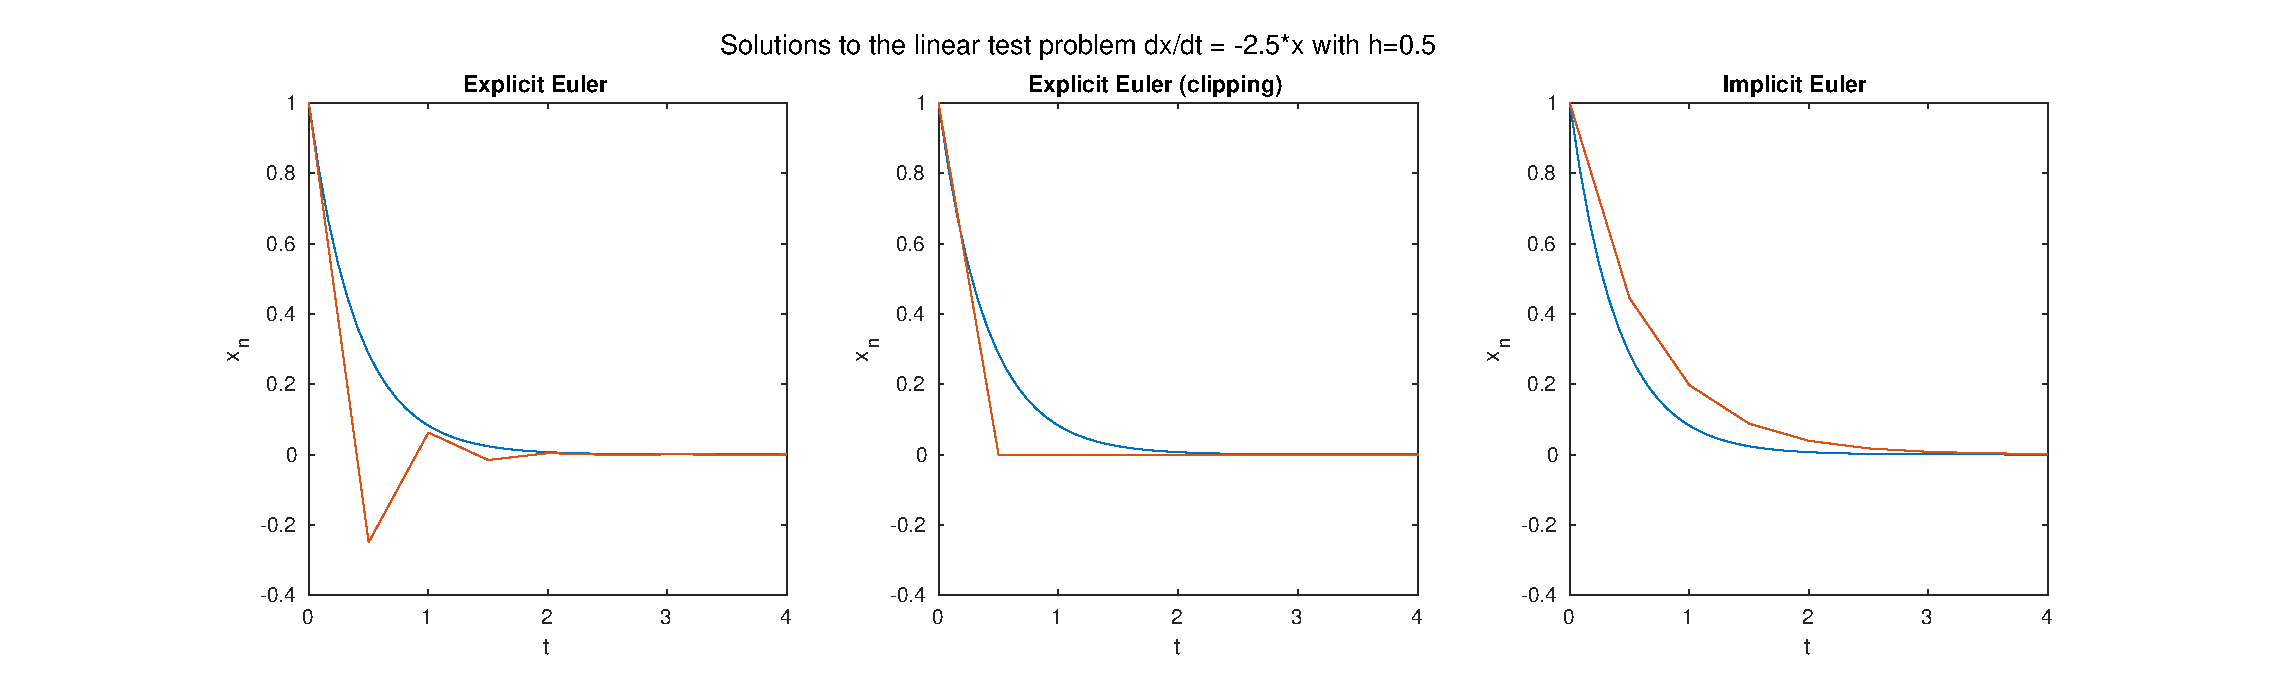
\includegraphics[width=0.75\linewidth]{Matlab/clippingisbad.eps}
    \caption{
        Comparison of methods applied to the linear test problem.
        True solution is marked in blue on each plot.
    }
    \label{fig:eulertriple}
\end{figure}

Before considering the problem of positivity preserving methods in depth, we will first consider the method which we will refer to as ``fixing'' or ``clipping''.
We use the forward Euler method $x_{i+1} = x_i + hf(x_i)$, except at every step we perform a fix by considering every entry in $x_i$ and if it is negative, we just set it to zero.
We can write this formally as the method
\begin{align*}
    x_{i+1} &= x_i + h f(x_i) \\
    x_{i+1} &= \mathcal{H}_+(x_{i+1}) 
\end{align*}
where $\mathcal{H}_+$ is the thresholder that sets all negative entries to zero.
This is equivalent to a projection of $x$ to a vector subspace of lower dimension, determined by in which dimensions $x$ is positive.

This method is very cheap, and it preserves positivity, so it seems like an easy choice.
The fixing step to eliminate negative entries can be applied in general to any numerical method.
See Figure \ref{fig:eulertriple}, where we have compared regular explicit Euler, explicit Euler with clipping, and implicit Euler methods applied to the linear test problem.
Regular Euler's method fails to preserve positivity unconditionally, while the clipping method adjusts negative solutions to zero.
Backward Euler appears to preserve positivity.
%discuss a result

Euler's method serves as a useful baseline to demonstrate experimental ideas.
Being a first-order accurate method, it does not serve as an effective choice for general applications.
We will instead look at different approaches to preserving positivity of the numerical solution,
using the graph-Laplacian structure explored earlier.

\subsection{General Solutions}

Consider the problem $\dot{x} = Ax$, with initial condition $x(t=0) = x_0$, with a constant square matrix $A$.
The general solution to this problem is
\begin{equation*}
    x(t) = \mathrm{e}^{tA} x_0
\end{equation*}
where the matrix exponential is analogised from the scalar case
\begin{equation*}
    \mathrm{e}^A = I + A + \frac{1}{2}A^2 + \frac{1}{6}A^3 + \mathellipsis = \sum_{j=0}^{\infty} \frac{A^j}{j!}.
\end{equation*}
We have shown that in the case where $A$ is graph-Laplacian, solutions preserve positivity.

We can't immediately apply this exponential solution to the problem $\dot{x} = A(x)x$ because of the non-linear right hand side, which will lead to a different expansion via. product rule.
To see why, we will demonstrate the expansion. Assume that the solution for the graph-Laplacian problem is $x(t) = \exp(tA(x))x_0$.
Then
\begin{equation*}
    \dot{x} = \frac{\mathrm{d}}{\mathrm{d}t} \left(
        \mathrm{e}^{A(x)t}x_0 
    \right) = \frac{\mathrm{d}}{\mathrm{d}t} \left[
        A(x)t
    \right] \mathrm{e}^{A(x)t}x_0 = \left[
        A(x) + t A'(x) A(x) x
    \right] x
\end{equation*}
which does not satisfy the problem.
Note that this expension involves a derivative of $A(x)$. More on this later.

\subsection{Exponential Euler's Method and Matrix-Vector Taylor Series}

We said that we can't apply the exponential solution $x(t) = \exp(tA)x_0$ to the problem $\dot{x} = A(x)x$.
We will show this by demonstrating what happens if we do. We propose a method of the form
\begin{equation}
    x_{n+1} = \mathrm{e}^{h A(x_n)}x_n.
\end{equation}
This method fixes $A$ for each step. Therefore, one step is equivalently providing the analytical exponential solution to the problem $\dot{x} = A(y)x$,
where $y = x(t=0) = x_n$.
In our scope of analysis we will call this the ``exponential Euler method'', due to its similarity to the classic method.
Considering the true solution after a timestep, we want to find an expression for the \textit{truncation error}.
We write $x(t_n) = x_n$ at the current step and look at the difference between $x(t_n + h)$ (the true value) and $x_{n+1}$ (the method).
However, first we need to consider the Taylor expansion on $x(t + h)$
\begin{equation*}
    x(t+h) = x(t) + h \dot{x}(t) + \frac{h^2}{2}\ddot{x}(t) + \mathellipsis
\end{equation*}
which involves derivatives of the nonlinear vector function $A(x)x$
\begin{equation*}
    x(t+h) = x + h A(x)x + \frac{h^2}{2} \left[ A'(x)A(x)xx + A(x)^2  x \right] + \mathcal{O}(h^3)
\end{equation*}
writing $x = x(t)$.
As we can see, this involves derivatives of $A(x)$, and associativity of matrix multiplication breaks.
To clarify, multiplication following from left to right should always perform defined operations.
Derivatives of $A(x)$ are rank-incrementing tensors: since $A \in \mathds{R}^{d \times d}$,
the first derivative is $A'(x) \in \mathds{R}^{d \times d \times d}$.
The $k$-th order derivative satisfies $A^{(k)}(x) \in \mathds{R}^{d^{k+2}}$.
This analysis is essential for deriving the order of methods for problems of the form we are working with.

Evaluating the truncation error of the exponential Euler method gives us the expression
\begin{equation*}
    \begin{aligned}
        \tau(h) = x(t_n + h) - x_{n+1} &= x(t_n + h) - \mathrm{e}^{h A(x_n)}x_n \\
        &= x(t_n) + h \dot{x}(t_n) + \frac{h^2}{2}\ddot{x}(t_n) + \mathcal{O(h^3)} - \mathrm{e}^{h A(x_n)}x_n \\
        &= x_n + h A(x_n)x_n + \frac{h^2}{2}\left( A'(x_n)A(x_n)x_n x_n + A(x_n)^2 x_n \right) + \mathcal{O}(h^3)\\
         &- \left( I + h A(x_n) + \frac{h^2}{2}A(x_n)^2 + \mathcal{O}(h^3) \right)x_n \\
        &= \frac{h^2}{2} \left( A'(x_n) A(x_n) x_n x_n \right) + \mathcal{O}(h^3)
    \end{aligned}
\end{equation*}
hence the exponential Euler method is first order accurate.

\subsection{The Second-Order Strang Splitting Method}

The exponential Euler method involved considering the problem with one fixed component in order to apply the exponential solution.
We will consider the separation of components in more depth as in \cite{blanes_pos_2022} so that we can justify the construction of higher order methods.

We have the problem $\dot{x} = A(x)x$. Introduce the variable $z$ where the initial conditions for $x$ and $z$ satisfy $x(t=0) = x_0 = z_0 = z(t=0)$.
We then write the problem in two parts as
\begin{align*}
    \dot{x} &= A(z)x \\
    \dot{z} &= A(x)z.
\end{align*}
By separating the problem into two, we are essentially solving the problem twice.
However, the way we have distributed $x$ and $z$ means we can decompose this into two separate problems where we solve one for $x$ and one for $z$.
The first problem is
\begin{equation}
    \label{eqn:split1}
    \begin{aligned}
        \dot{x} &= A(z)x \\
        \dot{z} &= 0
    \end{aligned}
\end{equation}
which has solution
\begin{align*}
    x(t) &= \mathrm{e}^{tA(z_0)}x_0 \\
    z(t) &= z_0
\end{align*}
while the second problem is of alternate form for $x$ and $z$
\begin{equation}
    \label{eqn:split2}
    \begin{aligned}
        \dot{x} &= 0 \\
        \dot{z} &= A(x)z
    \end{aligned}
\end{equation}
which has solution
\begin{align*}
    x(t) &= x_0 \\
    z(t) &= \mathrm{e}^{tA(x_0)}z_0.
\end{align*}
It may appear confusing as to why we split the problem into two parts.
We know that if a problem is given by $\dot{x} = A(x)x$ then its solutions preserve positivity.
We also know that if a problem is given instead by $\dot{x} = Ax$ for any constant matrix $A$, then it has general solution given by $x(t) = \exp(tA)x_0$.
Therefore, by splitting the problem into two problems on $x$ and $z$,
the solutions are given by the exponential form since the matrices are fixed in each problem,
and the solutions preserve positivity because the matrices are of graph-Laplacian form.
Therefore these solutions preserve positivity \cite{blanes_pos_2022}, which we can use to begin constructing methods which maintain this.

The primary method given in \cite{blanes_pos_2022}, which is a solution to Equations \ref{eqn:split1} and \ref{eqn:split2} is given by the equations
\begin{equation}
    \begin{aligned}
        x_{n+\frac{1}{2}} &= \exp \left( \frac{h}{2} A(z_n) \right) x_n \\
        z_{n+1} &= \exp \left( h A(x_{n+\frac{1}{2}}) \right) z_n \\
        x_{n+1} &= \exp \left( \frac{h}{2} A(z_{n+1}) \right) x_{n+\frac{1}{2}}.
    \end{aligned}
    \label{eqn:secondorderstrangsplittingmethod}
\end{equation}
The solution $x_n$, $z_n$ or $(x_n + z_n)/2$ is second order accurate. We perform a half step in $x$,
followed by a full step in $z$ and then a second half-step in $x$, similar to Verlet integration.
In \cite{blanes_pos_2022}, it is stated that $|x_n - z_n|$ can be used as an estimate of the truncation error, for the method to be used adaptively with a variable time step. 

%order results from this method
%example comparing some methods
%magnus method
We will provide our own analysis on this method, by producing our own results on the truncation error of these methods.
First, we evaluate the truncation error of $z$. The whole numerical method can be written compactly by writing the explicit expression for $x_{n+\frac{1}{2}}$ inside the term.
Denote $x := x(t_n)$ and $A := A(x)$ for compactness, also $A' := A'(x)$ and the same generalised for any derivatives.
For an attempt of ease of notation, square brackets contain objects which are matrices or higher rank tensors, while parentheses contain objects which are vectors.
We can begin by writing the stage directly as
\begin{equation*}
    z_{n+1} = \exp \left[ h A \left( \exp \left( \frac{h}{2} A(z_n) \right) x_n \right) \right] z_n
\end{equation*}
and we note that $x_n = z_n = x(t_n)$, so we can swap every $z+n$ for $x$.
In full,
\begin{equation}
    z_{n+1} = \exp \left[ h A \left( \exp \left( \frac{h}{2} A(x) \right) x \right) \right] x.
    \label{eqn:strangz}
\end{equation}
Now start evaluating the truncation error.
\begin{align*}
    x(t_n + h) - z_{n+1} &= x(t_n+h) - \exp \left[ h A \left( \exp \left[ \frac{h}{2}A \right]x \right) \right]x \\
    &= x(t_n + h) - \left[
        I + h \left[ A \left( \exp \left[ \frac{h}{2}A \right]x \right) \right] \right. \\
        &+ \frac{h^2}{2} \left[ A \left( \exp \left[ \frac{h}{2}A \right]x \right) \right]^2 \\
        &+ \frac{h^3}{6} \left. \left[ A \left( \exp \left[ \frac{h}{2}A \right]x \right) \right]^3
    \right]x + \mathcal{O}(h^4).
\end{align*}
The inner term needs to be expanded out
\begin{align*}
    A\left( \exp \left[ \frac{h}{2}A \right]x \right) &= A \left( \left[ I + \frac{h}{2}A + \frac{h^2}{8}A^2 \right]x \right) + \mathcal{O}(h^3) \\
    &= A\left( x + \frac{h}{2}Ax + \frac{h^2}{8}A^2 x \right) + \mathcal{O}(h^3) \\
    &= A + A' \cdot \left( \frac{h}{2} Ax + \frac{h^2}{8} A^2 x \right) + A''(x) \left( \frac{h^2}{8}AxAx \right) + \mathcal{O}(h^3) \\
    &= A + \frac{h}{2}A'Ax + \frac{h^2}{8} \left( A' A^2 x + A'' Ax Ax \right) + \mathcal{O}(h^3).
\end{align*}
Note that an internal expansion leads to a big-O term inside the brackets,
which we can take outside the brackets by Taylor expansion centred at the collection of terms before the big-O expression.
If we plug this back in, the terms expand as
\begin{align*}
    &x(t_n + h) - \left[ I + h \left[ A + \frac{h}{2}A' A x + \frac{h^2}{8} \left[ A' A^2 x + A'' Ax Ax \right] \right] \right. \\
    &~~ + \left. \frac{h^2}{2} \left[ A + \frac{h}{2}A'Ax \right]\left[ A + \frac{h}{2}A'Ax \right] + \frac{h^3}{6}A^3 \right] x + \mathcal{O}(h^4) \\
    &= x(t_n + h) - \left[ I + hA + \frac{h^2}{2} \left[ A' Ax + A^2 \right] \right. \\
    &~~ + \left. \frac{h^3}{8} \left[ A' A^2 x + A'' Ax Ax + 2A'AxA + 2AA'Ax + \frac{4}{3}A^3 \right] \right]x + \mathcal{O}(h^4) \\
    &= x(t_n + h) - \left( x + hAx + \frac{h^2}{2} \left( A' Axx + A^2x \right) \right. \\
    &~~ + \left. \frac{h^3}{8} \left( A' A^2 xx + A'' Ax Ax x + 2A'AxAx + 2AA'Axx + \frac{4}{3}A^3x \right) \right) + \mathcal{O}(h^4).
\end{align*}
We can evaluate the Taylor expansion for $x$ itself
\begin{equation}
    \begin{aligned}
        x(t_n + h) &= x + h \dot{x} + \frac{h^2}{2}\ddot{x} + \frac{h^3}{6}\dddot{x} + \mathcal{O}(h^4) \\
        &= x + hAx + \frac{h^2}{2}\left( A'Axx + A^2x \right) \\
        &~~ + \frac{h^3}{6} \left( A''AxAxx + A'A'A xxx + 2A'A^2 xx + A A' A xx + A^3 x \right) + \mathcal{O}(h^4).
    \end{aligned}
    \label{eqn:thirdorderexpansion}
\end{equation}
Written on its own, the expansion of $z_{n+1}$ is
\begin{equation}
    \begin{aligned}
        z_{n+1} &= x + h Ax + \frac{h^2}{2} \left( A' A xx + A^2 x \right) \\
        &~~~~~~ + \frac{h^3}{8} \left(
            A' A^2 xx + A'' Ax Ax x + 2 A' Ax Ax + 2 A A' A xx + \frac{4}{3}A^3 x
            \right) \\
        &~~~~~~ + \mathcal{O}(h^4)
    \end{aligned}
    \label{eqn:strangzpanda}
\end{equation}
By comparing terms, the truncation error of the $z$ component is
\begin{equation}
    \tau_z(h) = h^3 \left( \frac{1}{24}A''AxAxx + \frac{1}{6}A'A'A xxx + \frac{5}{24} A' A^2 xx - \frac{1}{12}A A' A xx - \frac{1}{4}A' Ax Ax \right) + \mathcal{O}(h^4).
    \label{eqn:strangtruncz}
\end{equation}
Now look at the truncation error provided by the $x$ part of the method.
We already have, from above, an expression for $z_{n+1}$ in terms of powers of $h$, which will make the evaluation easier.
Write the expression for $x_{n+1}$
\begin{equation*}
    x_{n+1} = \exp \left[ \frac{h}{2} A(z_{n+1}) \right] x_{n+\frac{1}{2}}
\end{equation*}
which is equivalently
\begin{equation}
    x_{n+1} = \exp \left[ \frac{h}{2} A(z_{n+1}) \right] \exp \left[ \frac{h}{2} A \right] x.
    \label{eqn:strangx}
\end{equation}
Expand the expression
\begin{align*}
    x_{n+1} &= \exp \left[
        \frac{h}{2}A \left( x + h Ax + \frac{h^2}{2} \left( A' A xx + A^2 x \right) + \mathcal{O}(h^3) \right)
    \right] \exp \left[
        \frac{h}{2}A
    \right] x \\
    &= \exp \left[
        \frac{h}{2}A + \frac{h}{2} A' \cdot \left( h Ax + \frac{h^2}{2}\left( A' A xx + A^2 x \right) \right)
    \right] \exp \left[
        \frac{h}{2}A
    \right] x + \mathcal{O}(h^4) \\
    &= \exp \left[
        \frac{h}{2}A + \frac{h^2}{2}A'Ax + \frac{h^3}{4} \left[ A' A' A xx + A' A^2 x \right]
    \right] \exp \left[
        \frac{h}{2}A
    \right] x + \mathcal{O}(h^4).
\end{align*}
Note that because of the $(h/2)$ scale, taking out the $\mathcal{O}(h^3)$ term by expansion leads to an $\mathcal{O}(h^4)$ term outside the expression.
This saves writing $z_{n+1}$ up to the order $h^3$ term, since it would not be included in the final expression up to order $\mathcal{O}(h^3)$.
Using the definition of the exponential for both parts, we get
\begin{align*}
    x_{n+1} &= \left[
        I + \left[ \frac{h}{2}A + \frac{h^2}{2} A' Ax + \frac{h^3}{4} \left[ A' A' A xx + A' A^2 x \right] \right] \right. \\
        &~~ + \frac{1}{2}\left[ \frac{h^2}{4}A^2 + \frac{h^3}{4} \left[ AA'Ax + A' AxA \right] \right] \\
        &~~ + \left. \frac{1}{6} \left[ \frac{h^3}{8}A^3 \right]
    \right] \times \left[
        I + \frac{h}{2}A + \frac{h^2}{8}A^2 + \frac{h^3}{48}A^3
    \right]x + \mathcal{O}(h^4).
\end{align*}
We have only included every term up to third order, and then taken all higher order terms outside of the expansions.
We can rearrange this into powers of $h$ to get
\begin{align*}
    x_{n+1} &= \left[
        I + \frac{h}{2}A + \frac{h^2}{8} \left[ 4A'Ax + A^2 \right] \right. \\
        &~~ + \left. \frac{h^3}{48}\left[ 12 A' A' A xx + 12 A' A^2 x + 6 A A' Ax + 6 A' AxA + A^3 \right] \right] \\
        &~~ \times \left[
        I + \frac{h}{2}A + \frac{h^2}{8}A^2 + \frac{h^3}{48}A^3
    \right]x + \mathcal{O}(h^4).
\end{align*}
Multiplying this expression, considering only terms up to third order, we get
\begin{align*}
    x_{n+1} &= \left[
        I + hA + \frac{h^2}{8} \left[ 4 A' Ax + 4A^2 \right]
    \right. \\
    &~~ + \left.
        \frac{h^3}{48} \left[ 12 A' A' A xx + 12 A' A^2 x + 6 A A' Ax + 6 A' Ax A + 2A^3  \right] + \frac{h^3}{16} \left[ 4 A' AxA + 2A^3 \right]
    \right]x \\
    &~~ + \mathcal{O}(h^4). 
\end{align*}
By collecting terms, simplifying, and multiplying through by $x$, we get the expression
\begin{equation}
    \begin{aligned}
        x_{n+1} &= x + h Ax + \frac{h^2}{2} \left( A' A xx + A^2 x \right) \\
        &~~~~~~ + \frac{h^3}{8} \left(
            2A'A'Axxx + 2 A' A^2 xx + A A' A xx + 3 A' Ax Ax + \frac{4}{3}A^3 x
            \right) \\
        &~~~~~~ + \mathcal{O}(h^4)
    \end{aligned}
    \label{eqn:strangxpanda}
\end{equation}
Comparing this to the true expansion from Equation \ref{eqn:thirdorderexpansion}, we can evaluate the truncation error $x(t_n + h) - x_{n+1}$ as
\begin{equation}
    \tau_x(h) = h^3 \left(
        \frac{1}{6}A'' Ax Ax x - \frac{1}{12}A' A' A xxx + \frac{1}{12} A' A^2 xx + \frac{1}{24}A A' A xx - \frac{3}{8}A A' A xx
    \right) + \mathcal{O}(h^4).
    \label{eqn:strangtruncx}
\end{equation}
We have obtained direct expressions for the truncation errors for both components of the splitting method.
Both expressions for truncation error, from Equations \ref{eqn:strangtruncz} and \ref{eqn:strangtruncx}, indicate that the method is second-order accurate.

The multiplication of the tensors as we have written them is not defined to satisfy associativity.
With the aim of relating the notation of Butcher \cite{butcher2016numerical}, we evaluate terms in the derivatives to provide some clarity.
We start with the definition of the system
\begin{equation*}
    \dot{x} = f(x) = A(x)x
\end{equation*}
We consider derivatives in the general case:
\begin{align*}
    \dot{x} &= f(x) \\
    \ddot{x} &= f'(x)\dot{x} = f'(x)f(x) = f'f \\
    \dddot{x} &= f''(x)f(x)f(x) + f'(x)f'(x)f(x) = f''(f,f) + f'f'f
\end{align*}
We can express terms for the derivatives just in $f$, which only go down to $x$ derivatives
\begin{align*}
    f(x) &= A(x)x = Ax \\
    f'(x) &= \frac{\partial f}{\partial x} = \frac{\partial}{\partial x} \left( A(x)x \right) = A'(x)x + A(x) = A'x + A \\
    f''(x) &= \frac{\partial}{\partial x} \left( A'(x)x + A(x) \right) = A''(x)x + A'(x) + A'(x) = A''x + 2A'
\end{align*}
and we can write the derivatives of $x$ in a way that resembles the convention
\begin{align*}
    \dot{x} &= f = Ax \\
    \ddot{x} &= f'f = \left[A'x + A\right] \left(Ax\right) \\
    \dddot{x} &= f''(f,f) + f'f'f = \left[ A''x + 2A' \right]\left( Ax, Ax \right) + \left[ A'x + A \right]\left[ A'x + A \right]\left( Ax \right)
\end{align*}
where $A''x + 2A'$ is a third rank tensor, $A'x + A$ is a matrix and $Ax$ is a vector.

We will now briefly consider statements from \cite{blanes_pos_2022} regarding the properties of the splitting method.
We have mentioned the authors' claim that the difference $|x_{n+1} - z_{n+1}|$ can be taken as an estimate of the error of the method.
Using the expansions in Equations \ref{eqn:strangzpanda} and \ref{eqn:strangzpanda}, we can write their difference as
\begin{equation}
    z_{n+1} - x_{n+1} = \frac{h^3}{8} \left(
        A'' Ax Ax x + A A' A xx - A' A^2 xx - A' Ax Ax - 2 A' A' A xx
    \right) + \mathcal{O}(h^4).
    \label{eqn:strangdiff}
\end{equation}
This expression on the difference between methods contains every expression in the truncation error for $z$ (Equation \ref{eqn:strangtruncz}), of which there are five.
This may motivate its use as an estimate of the error.
However on comparing the two, there is a difference of sign for three expressions, and no consistency of scaling.
The difference expression does not contain the term $AA'Axx$, which appears in the truncation error for $x$.

One potentially interesting component of this analysis comes from how the different stages eliminate different elements in the truncation errors.
We may be motivated to take a linear combination of $x_{n+1}$ and $z_{n+1}$ such that we can obtain a new truncation error which is, in some sense, minimised.
Arguments are given in the Appendix, since the method borrows from convex optimisation \cite{boyd2004convex} and is not entirely relevant to the discussion.
Particularly, the approach is similar to Ralston \cite{ralston1962runge}.
We find that the appropriate linear combination, of the form $y_{n+1} = \mu z_{n+1} + \lambda x_{n+1}$,
would be theoretically best for $\mu = 17/24, \lambda = 7/24$.

The author acknowledges that the majority of this analysis on the truncation error of the splitting method is limited, due to lack of understanding of the behaviour of the mathematical objects.
Improvements to the results could be made, given rules on the multiplication in order to make simplifications.
We were unable to locate or provide any sources on this topic.
The analysis is the best we could achieve in this context.
% at the end, acknowledge this could all be wrong "due to lack of information regarding the behaviour of the tensor objects that appear in this context"

\subsection{Example - A Linear Problem on Two Variables}

\begin{figure}
    \centering
    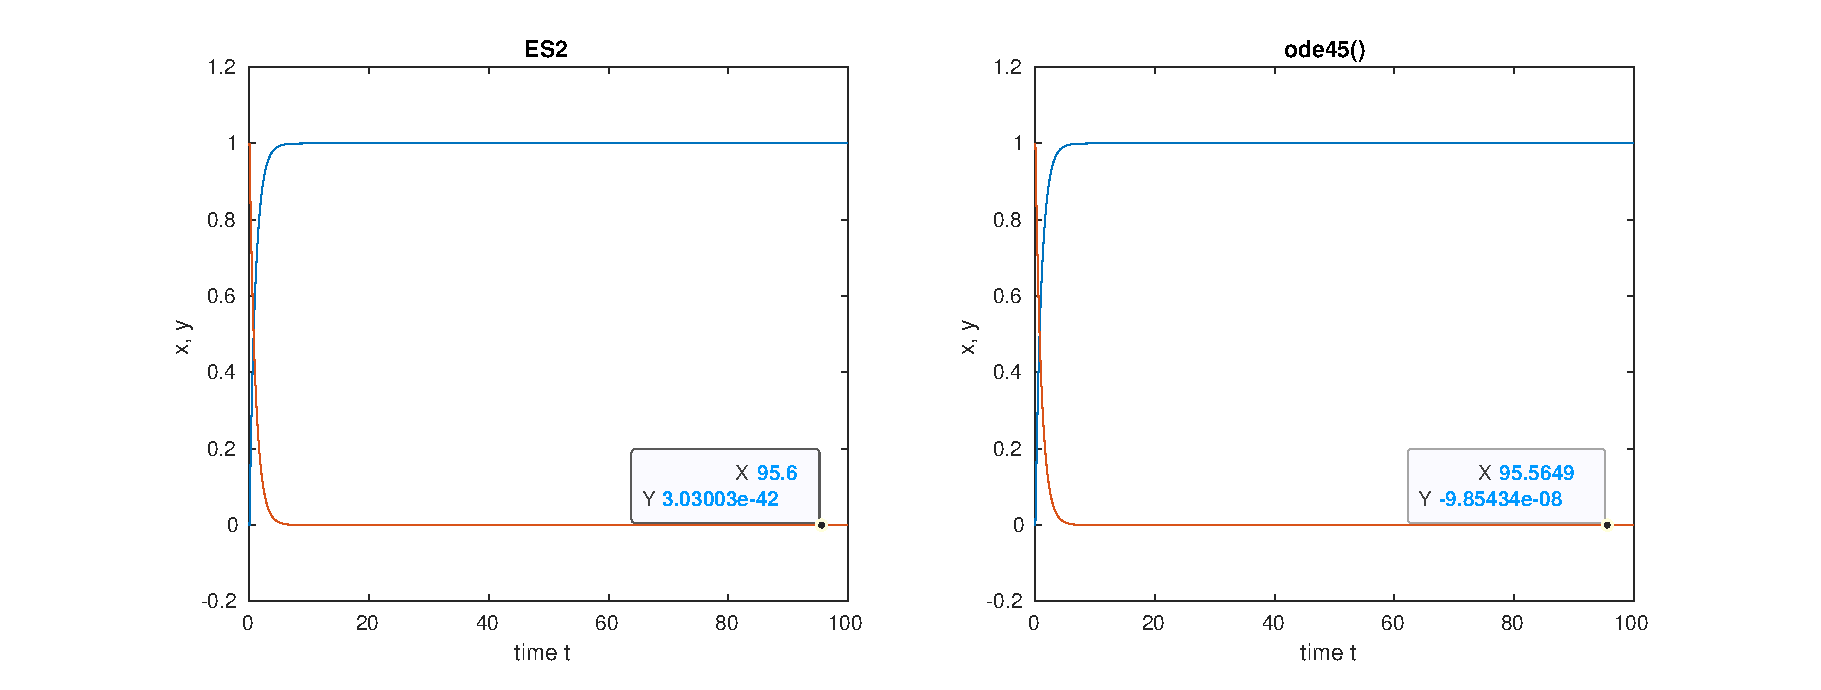
\includegraphics[width = \linewidth]{Matlab/linearproblempositivity.eps}
    \caption{
        Test problem on the system given by Equation \ref{eqn:alineartestproblem}.
        The left figure uses the "ES2" method given by Equation \ref{eqn:secondorderstrangsplittingmethod} taking its $x$ values as opposed to the $z$ values.
        ES2 preserves positivity of the solution throughout.
        The right figure uses MATLAB's \texttt{ode45()} integrator, with a reduced tolerance in order to break positivity.
        The values used were $a=0$ with initial condition $x_0 = 0$, $y_0 = 1$ running for a timespan up to $T = 100$.
        Confusingly the MATLAB graph indexes the horizontal axis $X$ and the vertical $Y$, whereas we plot $x$ and $y$ on the vertical axis against $t$.
        The point labels are necessary to indicate that the MATLAB integrator does not preserve positivity.
    }
    \label{fig:breakposlin}
\end{figure}

Consider the system given by
\begin{equation}
    \frac{\mathrm{d}x}{\mathrm{d}t} = y - ax,~~ \frac{\mathrm{d}y}{\mathrm{d}t} = ax - y
    \label{eqn:alineartestproblem}
\end{equation}
where $a$ is a given constant. This problem is explored briefly for demonstrative purposes in \cite{broekhuizen_biochem_2008}.
The problem admits formulation into the graph-Laplacian form
\begin{equation*}
    \frac{\mathrm{d}}{\mathrm{d}t}\begin{pmatrix}
        x \\
        y
    \end{pmatrix} = \begin{bmatrix}
        -a & 1 \\
        a & -1
    \end{bmatrix} \begin{pmatrix}
        x \\
        y
    \end{pmatrix}
\end{equation*}
where the matrix is constant.

A numerical solution is given in Figure \ref{fig:breakposlin}.
We show that a conventional explicit method, such as the Runge-Kutta method(s) applied in MATLAB's \texttt{ode45()} integrator does not unconditionally preserve positivity.
The formulation of the problem into graph-Laplacian form and the application of a nonnegative initial condition indicates that our solution should preserve positivity, but MATLAB's integrator does not maintain this.
Therefore we have shown that positivity may not be maintained by conventional integrators,
but it is succesful for the ES2 integrator which we know to unconditionally preserve positivity.

Implementation of ES2 with further testing is provided in Appendix \ref{apn:es2}.

\subsection{The Magnus Integrator}

An alternative method suggested in \cite{blanes_pos_2022} is the second order Magnus integrator.
We will first discuss the Magnus expansion \cite{Magnus_1954, blanesmagnus2009}, which allows us to construct this method.
The Magnus expansion considers the linear ODE given by
\begin{equation*}
    \dot{x} = A(t)x
\end{equation*}
with initial condition $x(t=0) = x_0$.
Since $A$ is not time-independent, the exponential solution we have discussed earlier does not hold.
We state that the problem is linear, but the time dependence analogises to the cases we have looked at for a matrix $A(x)$ or $A(t,x)$.
The Magnus expansion considers the solution of this problem to be of the form
\begin{equation*}
    x(t) = \exp(\Omega(t))x_0
\end{equation*}
for some matrix function $\Omega(t)$ which can be expressed in terms of the governing matrix $A$.
We write $\Omega(t)$ as an infinite sum over $\Omega_j(t)$ functions.
From the literature \cite{blanesmagnus2009}, we have formulae for these entries.
Specifically, we write
\begin{equation*}
    \begin{aligned}
        \Omega(t) &= \Omega_1(t) + \Omega_2(t) + \mathellipsis = \sum_{j = 0}^{\infty} \Omega_j (t) \\
        \Omega_1(t) &= \int_{0}^{t} A(\tau) \mathrm{d}\tau \\
        \Omega_n(t) &= \sum_{k=1}^{n-1} \frac{B_k}{k!} \int_{0}^{t} S_n^{(k)}(\tau) \mathrm{d}\tau \\
    \end{aligned}
\end{equation*}
where $B_k$ are the Bernoulli numbers \cite{bernoulli} and the $S_n^{(j)}$ matrices are defined
\begin{equation*}
    \begin{aligned}
        S_n^{(1)} &= [\Omega_{n-1}, A] \\
        S_n^{(n-1)} &= \operatorname{ad}_{\Omega_1}^{n-1}(A) \\
        S_n^{(j)} &= \sum_{m=1}^{n-j} \left[ \Omega_m, S_{n-m}^{(j-1)} \right] ~~ \text{for}~ 2 \le j \le n-1.
    \end{aligned} 
\end{equation*}
where $\left[\cdot, \cdot\right]$ is the matrix commutator $[A,B] = AB-BA$ and $\operatorname{ad}_A^{j} B = [ A, \operatorname{ad}_A^{(j-1)}B ]$ where $\operatorname{ad}_A^0 B = B$.
For clarity, the matrix integral is defined element-wise since $t$ is a scalar.
We truncate the Magnus expansion to attain an approximation of the solution to a particular order.
Taking just the first term $\Omega_1$, we obtain
\begin{equation*}
    x(t) = \exp\left( \int_{0}^{t} A(\tau) \mathrm{d}\tau \right)x_0
\end{equation*}
which we can approximate with a first order method to get
\begin{equation*}
    x_{n+1} = \exp\left( h A(t_n) \right)x_n.
\end{equation*}
Note that we are given $A = A(t)$ in the definition of the Magnus expansion,
while problems we are interested in have $A=A(x)$ or $A=A(x,t)$.
The use of the Magnus expansion is in being able to express the solution to the time-dependent matrix ODE as something computable.
By taking the first order term in the expansion and forming a first order approximation, we construct a first-order method which is the same as the ``exponential Euler method''  we saw earlier.
This outlines an idea for constructing better approximations, by taking higher order Magnus expansions and higher order approximations.

In \cite{blanes_pos_2022}, the second order Magnus solution is given by
\begin{equation*}
    x(t) = \exp \left[ \int_{0}^{t} A \left( e^{\tau A(x_0)} x_0 \right) \mathrm{d}\tau \right]x_0
\end{equation*}
for a problem with initial condition $x(t=0) = x_0$.
We can swap $x_0$ for $x_n$ and this provides the Magnus solution to second order at $t_n + h$,
which we then approximate to produce a numerical method.
Using the trapezium method by evaluating the integrand at both ends and taking the midpoint,
we obtain the method
\begin{equation*}
    x_{n+1} = \exp \left[ \frac{h}{2}\left[ A(x_n) + A\left(
        \exp \left[ h A(x_n) \right]x_n
    \right) \right] \right]x_n.
\end{equation*}
Alternatively, using the midpoint rule the method is given by
\begin{equation}
    x_{n+1} = \exp\left(h A \left( \exp\left(\frac{1}{2}h A(x_n)\right) x_n \right) \right) x_n.
    \label{eqn:secondordermagnus}
\end{equation}
We will consider the second order Magnus integrator as the approximation using the midpoint rule, which is the same options taken by the authors of \cite{blanes_pos_2022}.
The authors also provide more detail on the formulation for higher order methods.
Both the trapezium and midpoint rule approximations are second-order accurate.
More properties of the Magnus expansion are explored in \cite{blanesmagnus2009}.

The formulation of the second-order Magnus integrator (midpoint) is identical to the $z_{n+1}$ stage of the second order Strang splitting method for one step \cite{blanes_pos_2022}.
See Equation \ref{eqn:strangz} for the definition with Taylor-expanded form in Equation \ref{eqn:strangzpanda}.
See Equation \ref{eqn:strangtruncz} for the truncation error.

\subsection{Example - The MAPK Cascade}

\begin{figure}
    \centering
    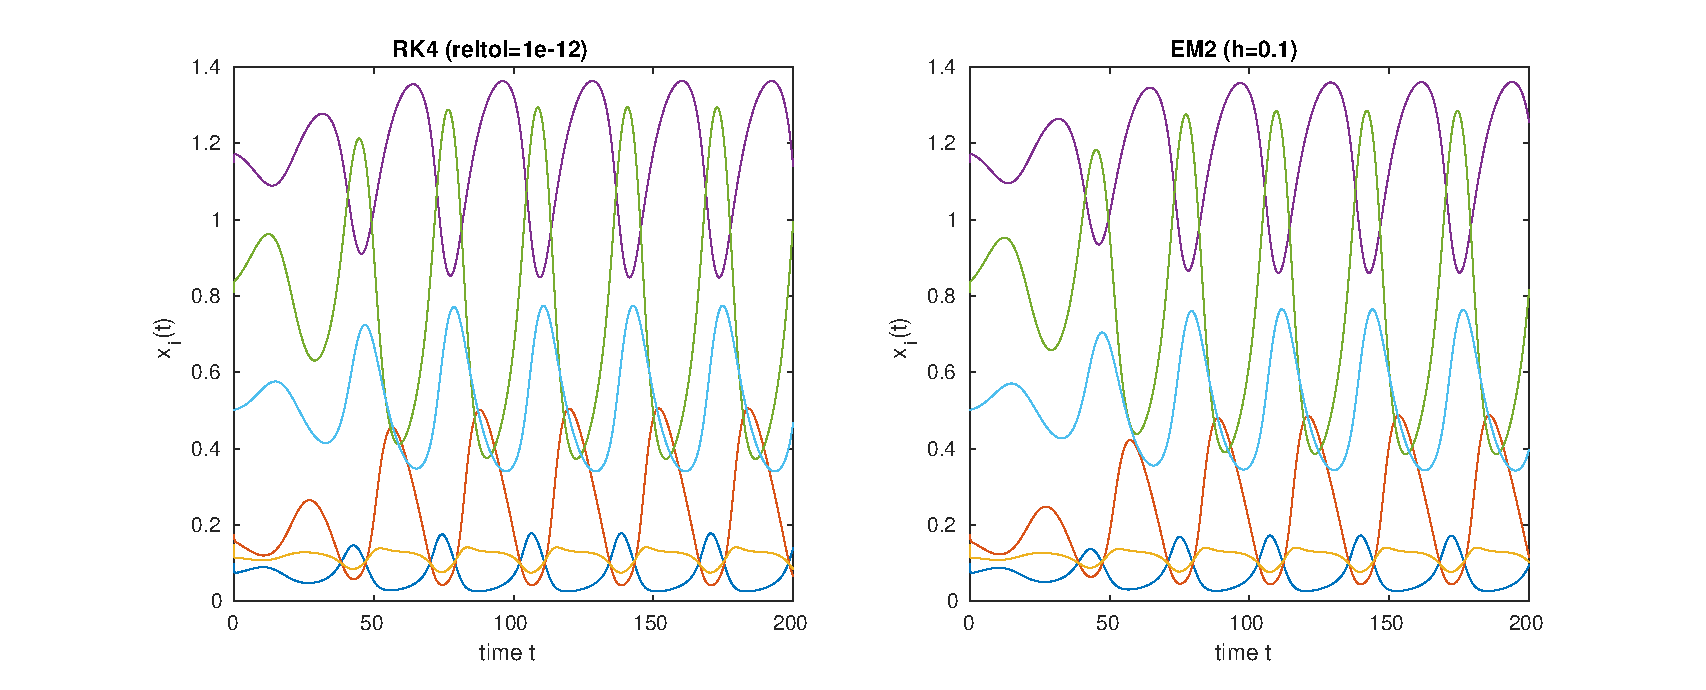
\includegraphics[width=\linewidth]{Matlab/mapkdual.eps}
    \caption{
        Graphic of the trajectories given by the MAPK cascade problem.
        The Runge-Kutta method applied by \texttt{ode45()} has a relative tolerance set to $10^{-12}$ which is extremely accurate.
        This gives us our best feasible approximation, to compare other methods to.
        This is shown in the left figure.
        The figure on the right shows the solution computed using the EM2 Magnus integrator, with a uniform step size of $h=0.1$.
        The variables $x_i$ are the concentrations of different chemical species involved in the reaction.
    }
    \label{fig:mapkdual}
\end{figure}

The Mitogen-activated protein kinase cascade (MAPK) model is an autonomous system on six variables,
given in the form of $\dot{x} = A(x)x$, where $A$ is given by
\begin{equation*}
    A(x) = \begin{bmatrix}
        -k_7 - k_1 x_2      & 0              & 0            & k_2  & 0    & k_6 \\
        0                   & -k_1 x_1       & k_5          & 0    & 0    & 0 \\
        0                   & 0              & -k_3 x_1-k_5 & k_2  & k_4  & 0 \\
        (1 - \alpha)k_1 x_2 & \alpha k_1 x_1 & 0            & -k_2 & 0    & 0 \\
        0                   & 0              & k_3 x_1      & 0    & -k_4 & 0 \\
        k_7                 & 0              & 0            & 0    & 0    & -k_6
    \end{bmatrix}.
\end{equation*}
The problem describes the behaviour of different chemical species involved in a biochemical reaction involving enzymes at a microcellular level \cite{hadavc2017mapk}. 
The form of this problem is taken from \cite{blanes_pos_2022}, which itself is modified from the properties discussed in \cite{hadavc2017mapk}.
The coefficients $k_j$ are given as $k_1 = 100/3, k_2 = 1/3, k_3 = 50, k_4 = 1/2, k_5 = 10/3, k_6 = 1/10, k_7 = 7/10$.
Note that the values involving the term $\alpha$ show that this graph does not admit graph-Laplacian structure as we have defined.
For $\alpha = 1$, the first column sum is zero but the second is not,
and for $\alpha = 0$ the opposite is true.
Furthermore the fourth column sum is never zero since we have defined $k_2$ to be non-zero.
This is addressed by \cite{blanes_pos_2022}, and we state that this problem adheres to the requirements of positivity preservation as long as $\alpha \in [0,1]$.
On inspection, this is the condition to require positivity of the entries involving $\alpha$, which themselves are not on the diagonal.
Hence this criteria is sufficient to guarantee positivity by the Theorem we stated earlier.
We take $\alpha = 0.1$ for our computations, acknowledging that any value in $[0,1]$ is suitable.

The MAPK cascade is an autonomous system which developes a sustained oscillation cycle.
See Figure \ref{fig:mapkdual} for a visualisation of the behaviour of the system.
We consider the EM2 integration method for solving this problem, with a time step of $h=0.1$.
We compare this with the output provided by MATLAB's \texttt{ode45()}, using a very low relative tolerance, which we consider the ``exact'' solution in a sense that we cannot obtain a better approximation.
The behaviours of both are extremely similar, however the implementation of EM2 has a recogniseable error, which we can most easily notice when the paths of the values intersect.
We can also make the assertion that EM2 preserves positivity for this problem, by inspection of the graph.
This result is consistent if we extend the timespan of the solution. 

Implementation of positivity preserving methods for this problem are provided in Appendix \ref{apn:aprx}


%Solving this problem with EM2. And the splitting method?

% next section is approximating the exponential
\section{Approximation of the Matrix Exponential}
%pade
%the first order approximation
%krylov methods
This section involves some linear algebra material which we have not covered.
A summary of the required information is given in the Appendix if needed.

\subsection{Challenges, series computation}
%mention instability for low N

The positivity preservation methods discussed so far all have one problem in common, being the use of the matrix exponential.
Computing the matrix exponential is significantly expensive, so we hope to introduce some form of approximation by which we can retain a given order of a method.
We might first think to compute the exponential directly from the definition \cite{higham2008exponential}:
\begin{equation*}
    \mathrm{e}^A = I + A + \frac{1}{2}A^2 + \frac{1}{6}A^3 + \mathellipsis = \sum_{j=0}^{\infty} \frac{A^j}{j!}.
\end{equation*}
If we are working in finite precision floating point arithmetic, we can assume that at some point the series will converge such that the sums to $n$ and $n+1$ are represented exactly the same \cite{moler2003dubious}.
In this case, we take the sum to $n$
\begin{equation*}
    \mathrm{e}^A \approx \sum_{j = 0}^{n} \frac{A^j}{j!}.
\end{equation*}
and using a modified Horner's form \cite{knuth2014art} we can express this as
\begin{align*}
	\sum_{j = 0}^{n} \frac{A^j}{j!} &= I + A + \frac{1}{2!}A^2 + \mathellipsis + \frac{1}{n!} A^n \\
	&= I + A\left(
	I + \frac{1}{2} A\left(
			I + \mathellipsis\left(
				\mathellipsis \left( I + \frac{1}{n} A
				\right)
			\right)
		\right)
	\right).
\end{align*}
There are $n$ matrix additions, $n-1$ divisions of a matrix by a scalar and $n-1$ matrix multiplications required to compute this expression.
A multiplication of two $d \times d$ matrices requires $\mathcal{O}(d^3)$\footnote{
    For computer algebra operations, a lower order is better because we often deal with large problems.
    In comparison, we want numerical methods to have higher order because $h$ is often very small.
} floating point operations.
Even with this improvement in efficiency, using this approach to compute a matrix exponential appears expensive.
We will now show that it is also unstable.

The following example is an adjustment of the first demonstration from \cite{moler2003dubious}.
Consider the matrix given by
\begin{equation*}
    A = \begin{bmatrix}
        -121 & 60 \\
        -160 & 79
    \end{bmatrix}.
\end{equation*}
Computing the series form of the exponential directly in double-precision arithmetic sums to $N = 139$ terms, and gives us the solution
\begin{equation*}
    \mathrm{e}_s^A = \begin{bmatrix}
        -2.6531 & -97.1835 \\
        -61.9581 & -184.0359
    \end{bmatrix}.
\end{equation*}
The true form of $A$ can be written as a conjugate transformation
\begin{equation*}
    A = \begin{bmatrix}
        1 & 3 \\
        2 & 4
    \end{bmatrix} \begin{bmatrix}
        -1 & 0 \\
        0 & -41
    \end{bmatrix} \begin{bmatrix}
        1 & 3 \\
        2 & 4
    \end{bmatrix}^{-1}.
\end{equation*}
and so the exponential can be written as 
\begin{equation*}
    \mathrm{e}^A = \begin{bmatrix}
        1 & 3 \\
        2 & 4
    \end{bmatrix} \begin{bmatrix}
        \mathrm{e}^{-1} & 0 \\
        0 & \mathrm{e}^{-41}
    \end{bmatrix} \begin{bmatrix}
        1 & 3 \\
        2 & 4
    \end{bmatrix}^{-1} \approx \begin{bmatrix}
        -0.7358 & 0.5518 \\
        -1.4715 & 1.1036
    \end{bmatrix}.
\end{equation*}
Clearly the exponential computed via series approximation is not an adequate estimate.
% explain the error. moler claims that terms in the sum have magnitudes greater than machine precision of opposite signs, so when adding them we gain terms greater than the final result.

% also mention low order approximations, where norms can cause trouble

Since this implementation is clearly inadequate, we look for alternative methods for computing the matrix exponential.

\subsection{The Pad\'e Approximation, Scaling and Squaring}

\begin{figure}
    \centering
    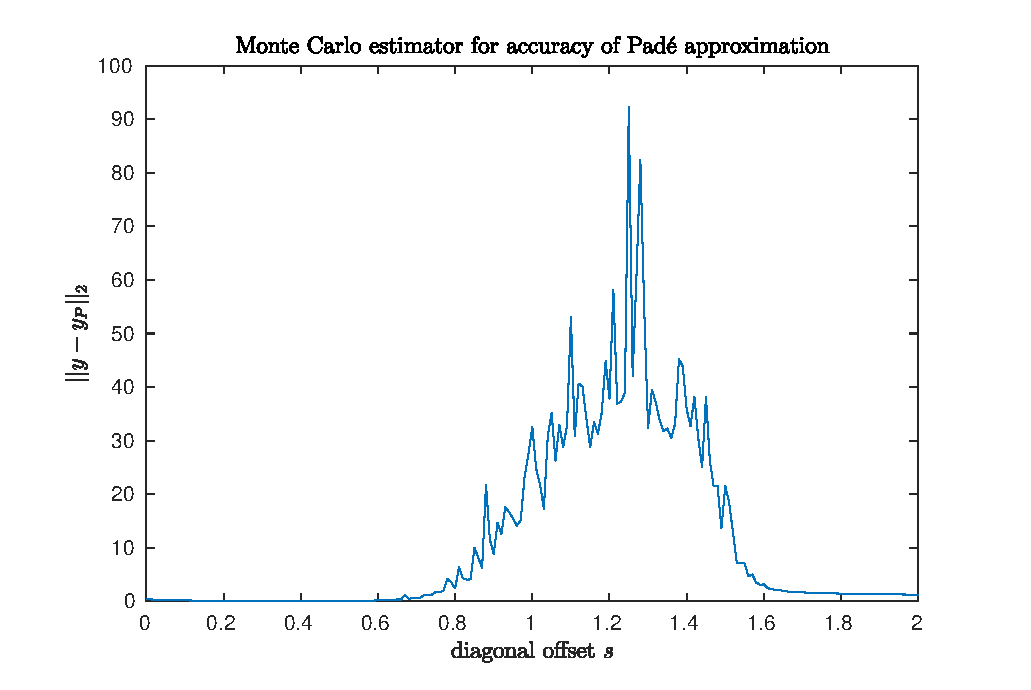
\includegraphics[width=0.65\linewidth]{Matlab/padeapproximator.eps}
    \caption{
        A Monte-Carlo estimate to evaluate the error of the Pad\'e approximation of the matrix exponential.
        For each value of $s$ in the interval $[0,2]$, we generate a sample of random $10\times 10$ graph-Laplacian matrix and positive vector pairs with entries uniformly distributed on $[0,1]$,
        then evaluate the $2$-norm error between $\exp(A)x$ using the MATLAB \texttt{expm()} function, and the Pad\'e approximation $Q^{-1}Px$.
        However, we use the decomposition $A = \bar{A} + \hat{a}I$ and define $\hat{a}= -s |\max(a_{ii})|$.
        We use the Pad\'e method to estimate $\exp(\bar{A})$ where its diagonal is modified from $A$ depending on $s$.
        If $s \ge 1$ then $\bar{A}$ is entirely nonnegative, whereas if $s<1$ then there is at least one negative entry on the diagonal of $\bar{A}$.
        This figure shows that there is an interval of values for $s$ such that it is unsuitable to take the Pad\'e approximation of $\bar{A}$. 
        The rough shape of the curve could come from the randomness of the sample matrices and vectors themselves.
    }
    \label{fig:mcpade}
\end{figure}

\begin{figure}
    \centering
    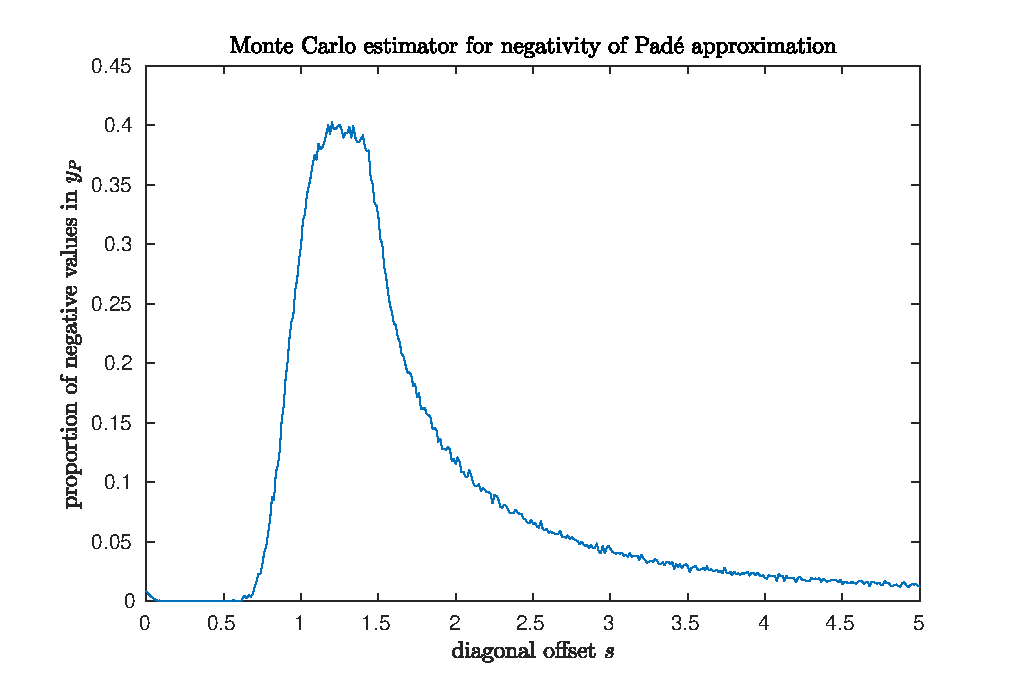
\includegraphics[width=0.65\linewidth]{Matlab/padenegativemc.eps}
    \caption{
        Monte-Carlo estimate for the negativity of the Pad\'e approximation of $\exp(A)x$.
        Uses the same configuration as Figure \ref{fig:mcpade}, the only difference being the evaluation of the dependent variable.
        We can identify a region of small $s$ for which the approximation appears suitable for preserving positivity.
        Not indentifiable from the previous figure is the slow descent as $s$ increases, implying that these values are not suitable despite showing low error before.
        The improved smoothness of this curve could imply that the behaviour of the negativity is inherent to the approximation.
    }
    \label{fig:mcpadeneg}
\end{figure}

Recall the Pad\'e approximation to the matrix exponential, which we explored when looking at symplectic and A-stable Runge-Kutta methods in Chapter \ref{cha:ham}.
We generalise this concept to functions on matrices. Given a function $f(A)$, there is a unique $[n,m]$ Pad\'e approximant \cite{higham2008exponential} $R_{mn}(A)$ given by the pair $P_{nm}(A), Q_{nm}(A)$ and formed by $R_{nm}(A) = \left[Q_{nm}(A)\right]^{-1}P_{nm}(A)$.
We will refer to $P$ as the numerator matrix and $Q^{-1}$ as the denominator matrix.
Formulae for Pad\'e approximants for certain matrix functions are known, such as the exponential. 
When computing the product $Q^{-1}P$ we always use a method to solve the system $QX=P$ rather than directly computing the inverse and product.

We said that formulae for the Pad\'e approximation for the exponential are known. From \cite{moler2003dubious, higham2008exponential} again, we have
\begin{equation}
    \begin{aligned}
        P_{nm}(A) &= \sum_{j=0}^{n} \frac{(n+m-j)!n!}{(n+m)!j!(n-j)!}A^j \\
        Q_{nm}(A) &= \sum_{j=0}^{m} \frac{(n+m-j)!m!}{(n+m)!j!(m=j)!}(-A)^j.
    \end{aligned}
\end{equation}
This is the approximant at zero.
A general Pad\'e approximant is taken about a point, such that it is equal to the approximated function at that point, similar to a Taylor expansion.
In some cases we might take the approximant about a different point, but here zero is no less suitable than anywhere else.

In \cite{blanes_pos_2022} it is stated that the second order diagonal Pad\'e approximation to the exponential is positivity preserving.
This is not true and we will provide a counterexample, alongside an investigation regarding how the approximation can be adjusted to preserve positivity.
The $[1,1]$ Pad\'e approximation to the exponential of $A$ is
\begin{equation*}
    D_{11}(A) = \left[ I - \frac{1}{2}A \right]^{-1} \left[ I + \frac{1}{2} A\right].
\end{equation*}
Consider the matrix given by
\begin{equation*}
    A = \begin{bmatrix}
        -4 & 1 & 0 \\
        2 & -1 & 2 \\
        2 & 0 & -2
    \end{bmatrix}
\end{equation*}
and vector
\begin{equation*}
    x = \begin{bmatrix}
        3 \\
        1 \\
        2
    \end{bmatrix}.
\end{equation*}
Clearly $A$ is graph-Laplacian and $x$ is positive.
To four significant figures the product of the exponential with the vector is
\begin{equation}
    \mathrm{e}^{A} x = \begin{pmatrix}
        0.9422 \\
        3.8506 \\
        1.2071
    \end{pmatrix}
\end{equation}
so positivity is preserved. However if we compute the $[1,1]$ Pad\'e approximant and compute the product we obtain
\begin{equation*}
    \left[D_{11}(A)\right]x = \left[ I - \frac{1}{2}A \right]^{-1} \left[ I + \frac{1}{2}A \right] x = \begin{pmatrix}
        -0.0167 \\
        1.1500 \\
        0.3667
    \end{pmatrix}
\end{equation*}
where we fail to preserve positivity.
A method is proposed in which we exploit the properties of the exponential by writing $A = \bar{A} + \hat{a}I$, such that $\bar{A}$ is entirely nonnegative.
Then
\begin{equation*}
    \mathrm{e}^A = \mathrm{e}^{\bar{A} + \hat{a}I} = \mathrm{e}^{\hat{a}} \mathrm{e}^{\bar{A}}
\end{equation*}
and we compute the $[1,1]$ Pad\'e approximant for $\bar{A}$.
In our example $\hat{a} = -4$ and
\begin{equation*}
    \mathrm{e}^{\hat{a}} [D_{11}(\bar{A})] x = \begin{bmatrix}
        0.5833 \\
        1.7500 \\
       -0.8333
    \end{bmatrix}.
\end{equation*}
So clearly the second order Pad\'e method does not preserve positivity.

There is one result which we can utilise in order to ensure positivity.
\begin{lemma}[Series Inverse \cite{horn2012matrix}]
    \label{lem:positiveinverse}
    If $A$ is a matrix which satisfies $||A||_2 < 1$, assuming $I-A$ is invertible we can write the inverse of $[I-A]$ as
    \begin{equation*}
        \left[ I - A \right]^{-1} = \sum_{k=0}^{\infty} A^k.
    \end{equation*}
\end{lemma}
\begin{proof}
    The condition on the norm $||A||_2 < 1$ is required in order for the series to converge.
    Define the series up to $N$ by $U_N:$
    \begin{equation*}
        U_N := \sum_{k=0}^{N} A^k.
    \end{equation*}
    Then multiply $[I-A]$ by this series
    \begin{align*}
        U_N \left[ I-A \right] &= \left[ I + A + A^2 + \mathellipsis + A^{N-1} + A^N \right] \left[ I - A \right] \\
        &= [I-A] + \left[ A-A^2 \right] + \mathellipsis + \left[ A^{N-1} - A^N \right] + \left[ A^N - A^{N+1} \right] \\
        &= I + [A-A] + \left[ A^2 - A^2 \right] + \mathellipsis + \left[ A^N - A^N \right] - A^{N+1} \\
        &= I - A^{N+1}.
    \end{align*}
    As $N \rightarrow \infty$, $A^N$ tends to the zero matrix because $||A||_2 < 1$ as assumed.
    Hence this product converges to the identity and we have an expression for the inverse.
    Thus,
    \begin{equation*}
        \left[ I - A \right]^{-1} = \lim_{N\rightarrow \infty}U_N = \sum_{k=0}^{\infty} A^k.
    \end{equation*}
\end{proof}
This result is especially useful when considering the reduction $A = \bar{A} + \hat{a}I$.
We have $\bar{A}$ is entirely positive by definition.
If we also have this bound on the spectral norm of $\bar{A}$,
then we know that the inverse of $[I-\bar{A}]$ is the series on powers of $A$, all of which must be positive.
Therefore, the inverse of $[I-\bar{A}]$ is positive.
In this context, we can guarantee that this approximation is positivity preserving.
This also relates to the Pad\'e approximation - if this holds then the $[1,1]$ approximation has the numerator and denominator matrices both positive.
We will look at this later.

A possible explanation for the mistake in \cite{blanes_pos_2022} could be the alternative approximations the authors use.
Considering the step $h$, the diagonal Pad\'e approximation is the product of two matrices
\begin{equation*}
    \mathrm{e}^{hA} \approx \left[ I - \frac{h}{2} A \right]^{-1} \left[ I + \frac{h}{2}A \right].
\end{equation*}
The following will appear confusing due to the scaling of $h/2$ in both matrices, which is necessary to the Pad\'e approximation of $\exp(hA)$.
However all the comments are identical up to scaling.

We can guarantee positivity of the Pad\'e approximation if both the numerator and denominator matrices are entirely positive.
The denominator matrix is itself a first order approximation to the matrix exponential $\exp((h/2)A)$ and is in fact guaranteed to be positive (more on this later).
However the numerator matrix has no guarantee of positivity: if $\hat{a}$ is the entry in $A$ of maximum absolute value,
then this matrix has at least one negative entry for $h > 2/|\hat{a}|$.
For the example we have given, $\hat{a} = -4$ by inspection.
Alternatively, recall $A = \bar{A} + \hat{a}I$ and consider the second order approximation involving only $\bar{A}$.
This is the same as $\exp(A)$ up to scaling, as shown earlier.
Since $\bar{A}$ is entirely nonnegative the numerator matrix must be nonnegative.
However this time there is no condition on the positivity of the denominator matrix.
We can give an informal proof:
assume $\bar{A}$ is entirely positive, with at least one zero on the diagonal.
Then consider $I - h\bar{A}$. This has at least one positive entry on the diagonal, but only has entirely positive diagonal for $h$ less than $(\max(\bar{a}_{ii}))^{-1}$.
Entries in $I - h\bar{A}$ not on the diagonal will be negative. Assuming the bound is \textit{not} satisfied, there will be one row in $I - h\bar{A}$ which is entirely negative.
For example,
\begin{equation*}
    I - h\bar{A} = \begin{bmatrix}
        1 & - & - \\
        - & - & - \\
        - & - & ?
    \end{bmatrix}.
\end{equation*}
The `?' entry cannot be greater than $1$, it is only included for generality.
Now assume its inverse is entirely positive. This is the denominator matrix, so we are hoping this is true.
Consider their product:
\begin{equation*}
    \left[I - h\bar{A}\right] \left[I - h\bar{A}\right]^{-1} = \begin{bmatrix}
        1 & - & - \\
        - & - & - \\
        - & - & ?
    \end{bmatrix} \begin{bmatrix}
        + & + & + \\
        + & + & + \\
        + & + & +
    \end{bmatrix}
\end{equation*}
Consider their product. Because this is the product of a matrix and its inverse, it should form the identity matrix.
However we assumed that the $i$-th row in $[I - h\bar{A}]$ is negative, and the $i$-th column in its inverse is positive (because we assumed the whole matrix is positive).
Therefore the entry $ii$ of their product, which is the identity matrix, is either zero or negative. This is a contradiction since entry $ii$ of the identity matrix is $1$.
Therefore it is not guaranteed that $[I - h\bar{A}]$ to be positive.

The explanation for the error could lie in both approximations. If we are approximating $\exp{hA}$, then the denominator matrix is entirely positive, but we cannot say the same for the numerator.
If we instead use the decomposition $A = \bar{A} + \hat{a}I$ and take the exponenial of $\bar{A}$, then the numerator matrix is guaranteed to be positive but the denominator may be negative.

See Figure \ref{fig:mcpade} for a visualisation of the stability of computing the Pad\'e approximation.
By using different values of $\hat{a}$ in the decomposition $A = \bar{A} + \hat{a}I$ for the reduction $\exp(A) = \exp(\hat{a})\exp(\bar{A})$,
the diagonal of $\bar{A}$ may or may not have negative values.
Particularly, we define $\hat{a}= -s |\max(a_{ii})|$ using a positive scaling parameter $s$.
If $s\ge 1$ we are using the method proposed by the authors in \cite{blanes_pos_2022} to let $\bar{A}$ be strictly positive. 
We can clearly identify from the given figures that there are values of the scaling parameter for which the approximations are unsuitable, despite appearing as suitable from its introduction in the paper.
Figure \ref{fig:mcpadeneg} evaluates negativity, clearly isolating a region of scaling of $\hat{a}$ such that the approximation is accurate and positivity preserving.

In MATLAB, the matrix exponential can be computed using the \texttt{expm()} function.
This implementation is very stable, due to the implementation of the scaling and squaring method \cite{higham2005scaling,moler2003dubious}.
The implementation of scaling and squaring is motivated by the identity that
\begin{equation*}
	\mathrm{e}^A = \left[ \mathrm{e}^\frac{A}{r} \right]^r.
\end{equation*}
The method takes $r$ to be a given power of $2$, say such that an approximation of $\exp(A/r)$ is stable by $A/r$ having a norm bounded below a threshold \cite{higham2008exponential}, and then repeatedly squares the result to get an approximation for $\exp(A)$.
This process provides much more stability in using the Pad\'e approximation, or even the series definition, of the matrix exponential.

\subsection{A first-order approximation}
%why its positivity preserving

In our discussion of the Pad\'e approximation we looked at guaranteed positivity of particular approximations.
We will now discuss some stronger results, centred around the approximation
\begin{equation*}
    \mathrm{e}^{hA} = \left[
        I - hA
    \right]^{-1} + \mathcal{O}(h^2)
\end{equation*}
which is first-order accurate and guaranteed to be positivity preserving.
First, note that when looking at the Pad\'e approximation we considered the positivity of the approximation
\begin{equation*}
    \mathrm{e}^{hA} \approx \left[ I - \frac{h}{2}A \right]^{-1} \left[ I + \frac{h}{2}A \right].
\end{equation*}
What is interesting is that both $Q^{-1}$ and $P$ in this Pad\'e approximation are themselves first order approximations of $\exp((h/2)A)$.

Understanding the positivity of this approximation involves Gershgorin's theorem for the eigenvalues of a matrix.
\begin{theorem}[Gershgorin \cite{gershgorin1931uber, horn2012matrix}]
    The eigenvalues of a matrix $A$ lie in the union of the $n$ discs $\mathcal{D}_i$ where
    \begin{equation*}
        \mathcal{D}_i = \left\{ z \in \mathds{C}: |z - a_{ii}| \leq \sum_{
            j = 1, j \ne i
        }^{n} |a_{ij}| \right\}.
    \end{equation*}    
\end{theorem}
\begin{proof}
    Proof omitted, see \cite{horn2012matrix}, pages $389-390$. 
\end{proof}

Gershgorin's theorem is a very useful bound on the eigenvalues - the disc $D_i$ is centered at $a_{ii}$ and its radius is the sum of the absolute values of the non-diagonal entries in the rest of the column.
This means that for a graph-Laplacian matrix, the discs containing the eigenvalues are centered at negative values on the real axis, and because a graph-Laplacian matrix has a zero column sum, these discs are restrained to the left half of the complex plane.
% next I-tA and its inverse
Assume $A$ has eigenvalues $\lambda_i$. Assuming $h>0$, $I - hA$ has eigenvalues $1-h \lambda_i$.
Since the eigenvalues of the inverse matrix are the inverses of the eigenvalues,\footnote{
    For matrix $M$ and eigenpair $\mu, y$, $y = M^{-1} My = M^{-1} \mu y$ and divide by $\mu$.
} the eigenvalues of $[I-hA]^{-1}$ are $1/(1-h \lambda)$.
From Gershgorin's theorem, the eigenvalues of $A$ have negative real part,
so these eigenvalues of the first order exponential approximation belong to the strictly positive half of the complex plane. % this does not mean it works!
We know that $[I-hA]$ has positive diagonal entries and negative off-diagonal entries,
and we can use Gershgorin's theorem to show that the diagonal of $[I-hA]^{-1}$ must be positive.
The proof that this inverse is entirely positive is given in \cite{blanes_pos_2022}.

The positivity preserving methods from Equations \ref{eqn:secondorderstrangsplittingmethod}, \ref{eqn:secondordermagnus} retain positivity and second order when some of the matrix exponentials are replaced with this first order substitution.
We evaluate the truncation error of the second order Magnus integrator when substituting the inside exponential with an approximation.
We use (parentheses) to contain terms which evaluate to vectors . For terms which evaluate to matrices or higher order tensors we use [square brackets].
\begin{equation*}
    \begin{aligned}
        \tau_\mathrm{m}(h) &= x(t_n + h) - \exp \left[
            h A \left(
                \left[
                    I - \frac{h}{2}A(x_n)
                \right]^{-1} x_n
            \right)
        \right]x_n \\
        &= x(t_n + h) - \exp \left[
            h A \left(
                \left[
                    \exp \left(
                        \left[
                            \frac{h}{2}A(x_n) + \mathcal{O}(h^2)
                        \right] x_n
                    \right)
                \right] x_n
            \right)
        \right]x_n \\
    \end{aligned}
\end{equation*}
We consider the exponential term and how the internal Taylor expansion brings the $\mathcal{O}(h^2)$ term out of $A$
\begin{equation*}
    \begin{aligned}
        &~ \exp \left[
            h A \left(
                \left[
                    \exp \left(
                        \left[
                            \frac{h}{2}A(x_n)
                        \right] x_n
                    \right) + \mathcal{O}(h^2)
                \right] x_n
            \right)
        \right]x_n \\
        &= \exp \left[
            h A \left(
                \left[
                    \exp \left(
                        \left[
                            \frac{h}{2}A(x_n)
                        \right] x_n
                    \right)
                \right] x_n
            \right) + \mathcal{O}(h^3)
        \right]x_n
    \end{aligned}
\end{equation*}
We can take the $\mathcal{O}(h^3)$ out to show that this is clearly the regular second order Magnus method plus a remainder in $h^3$ and hence is second order.
We have already looked at the order of the second order Magnus integrator in its original form. 

\subsection{A Proposed Method using Series Expansion}

%unlimited figures
\begin{figure}
    \centering
    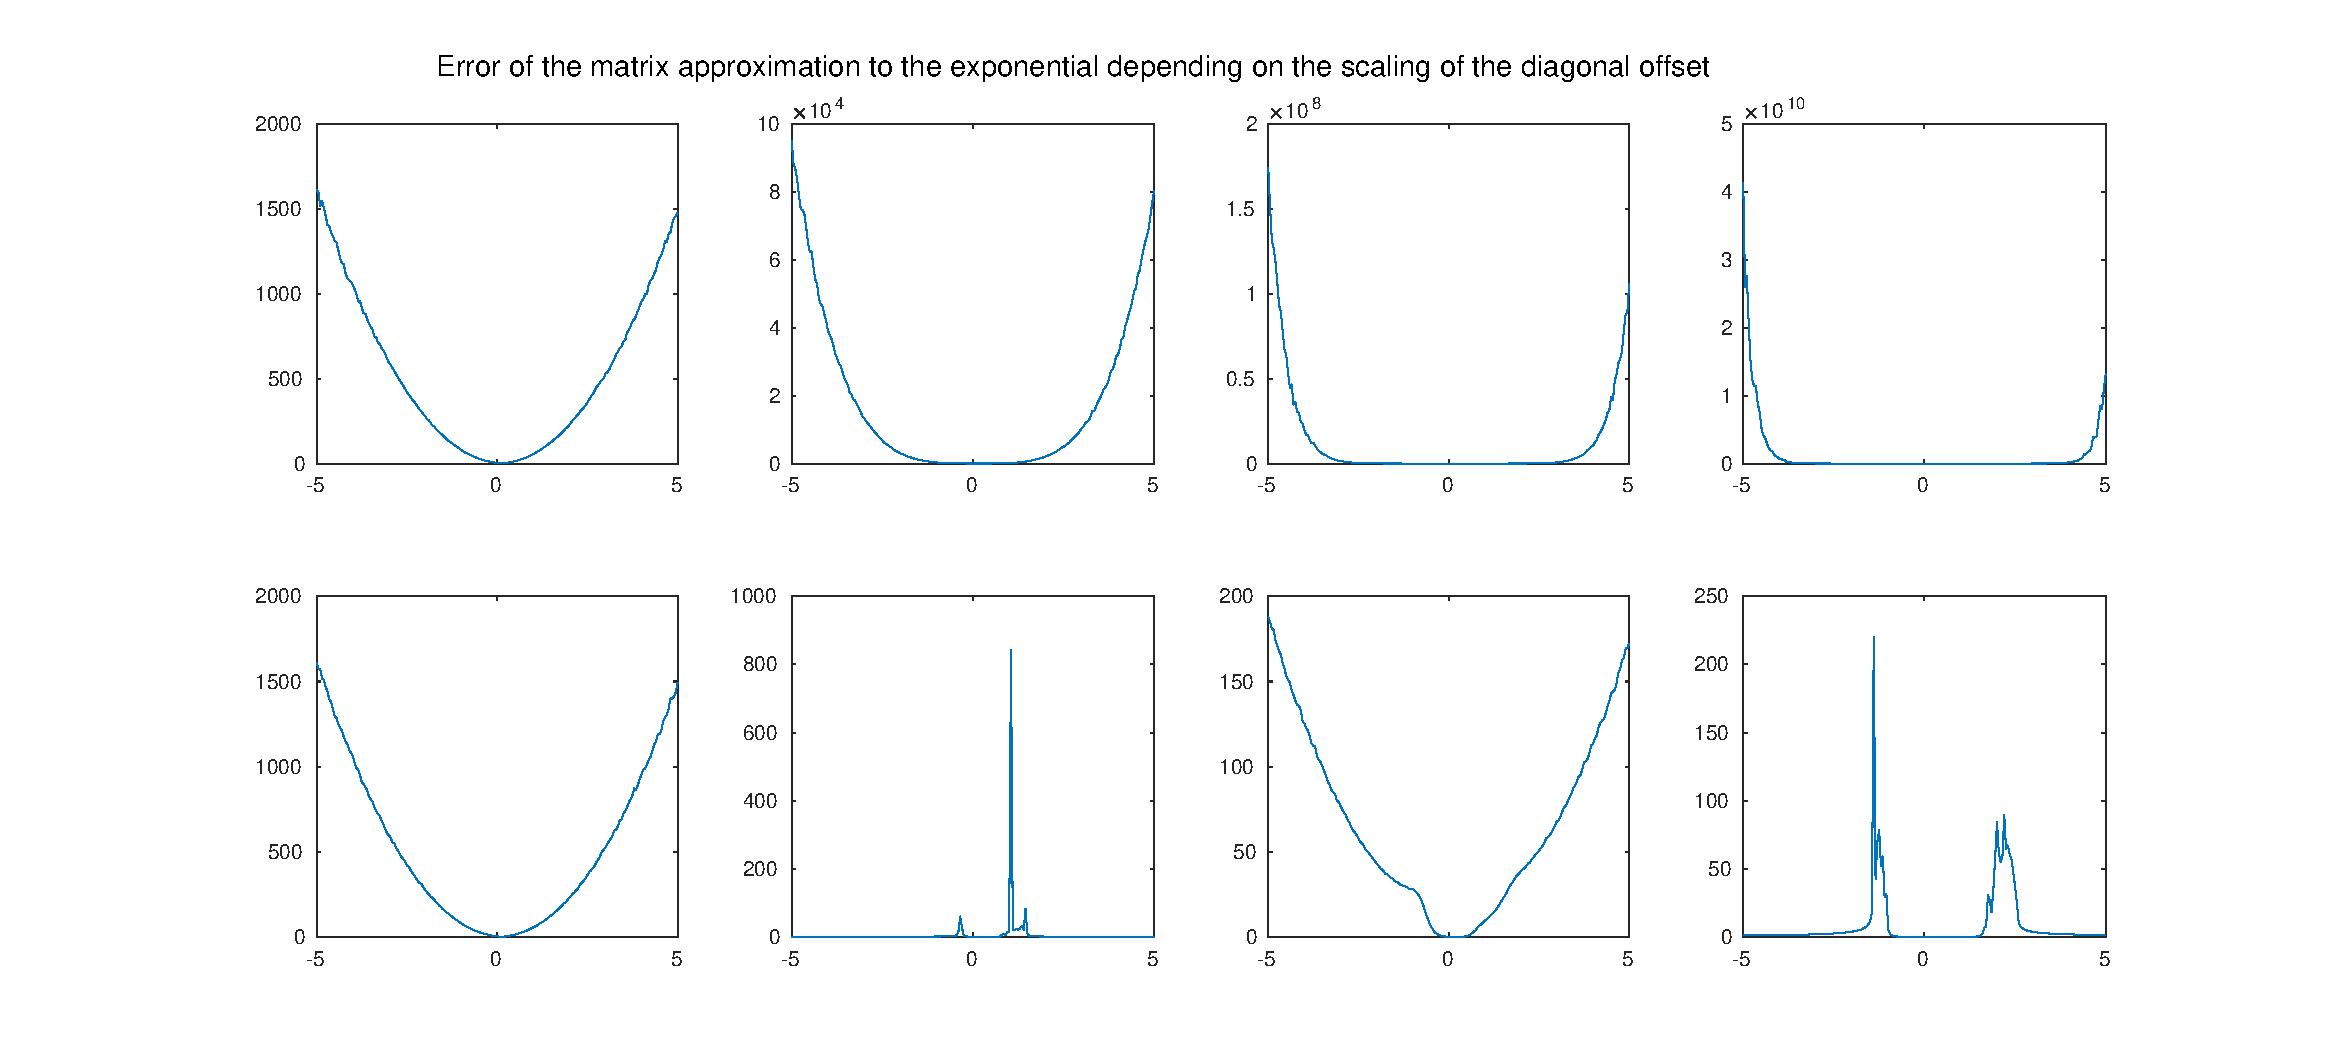
\includegraphics[width=\linewidth]{Matlab/padevsserieserr.eps}
    \caption{
        Comparison of how the scaling parameter for the diagonal offset, as seen in Figure \ref{fig:mcpade} affects the error of the approximation to the matrix exponential.
        The vertical axis is the evaluation of $||y-\bar{y}||_2$ where $\bar{y}$ is a Monte-Carlo estimate of $y = \exp(A)x$ using random $10 \times 10$ linear systems.
        The true value $y$ is evaluated using \texttt{expm()}.
        Top row: approximation using the series definition of the matrix exponential.
        Bottom row: approximation using the Pad\'e method.
        Column 1: first order (Pad\'e $[1,0]$) approximations.
        Column 2: second order (Pad\'e $[1,1]$) approximations.
        Column 3: fifth order (Pad\'e $[3,2]$) approximations.
        Column 4: tenth order (Pad\'e $[5,5]$) approximations.
        The diagonal Pad\'e methods maintain stability for large offset.
    }
    \label{fig:padeserieserr}
\end{figure}

\begin{figure}
    \centering
    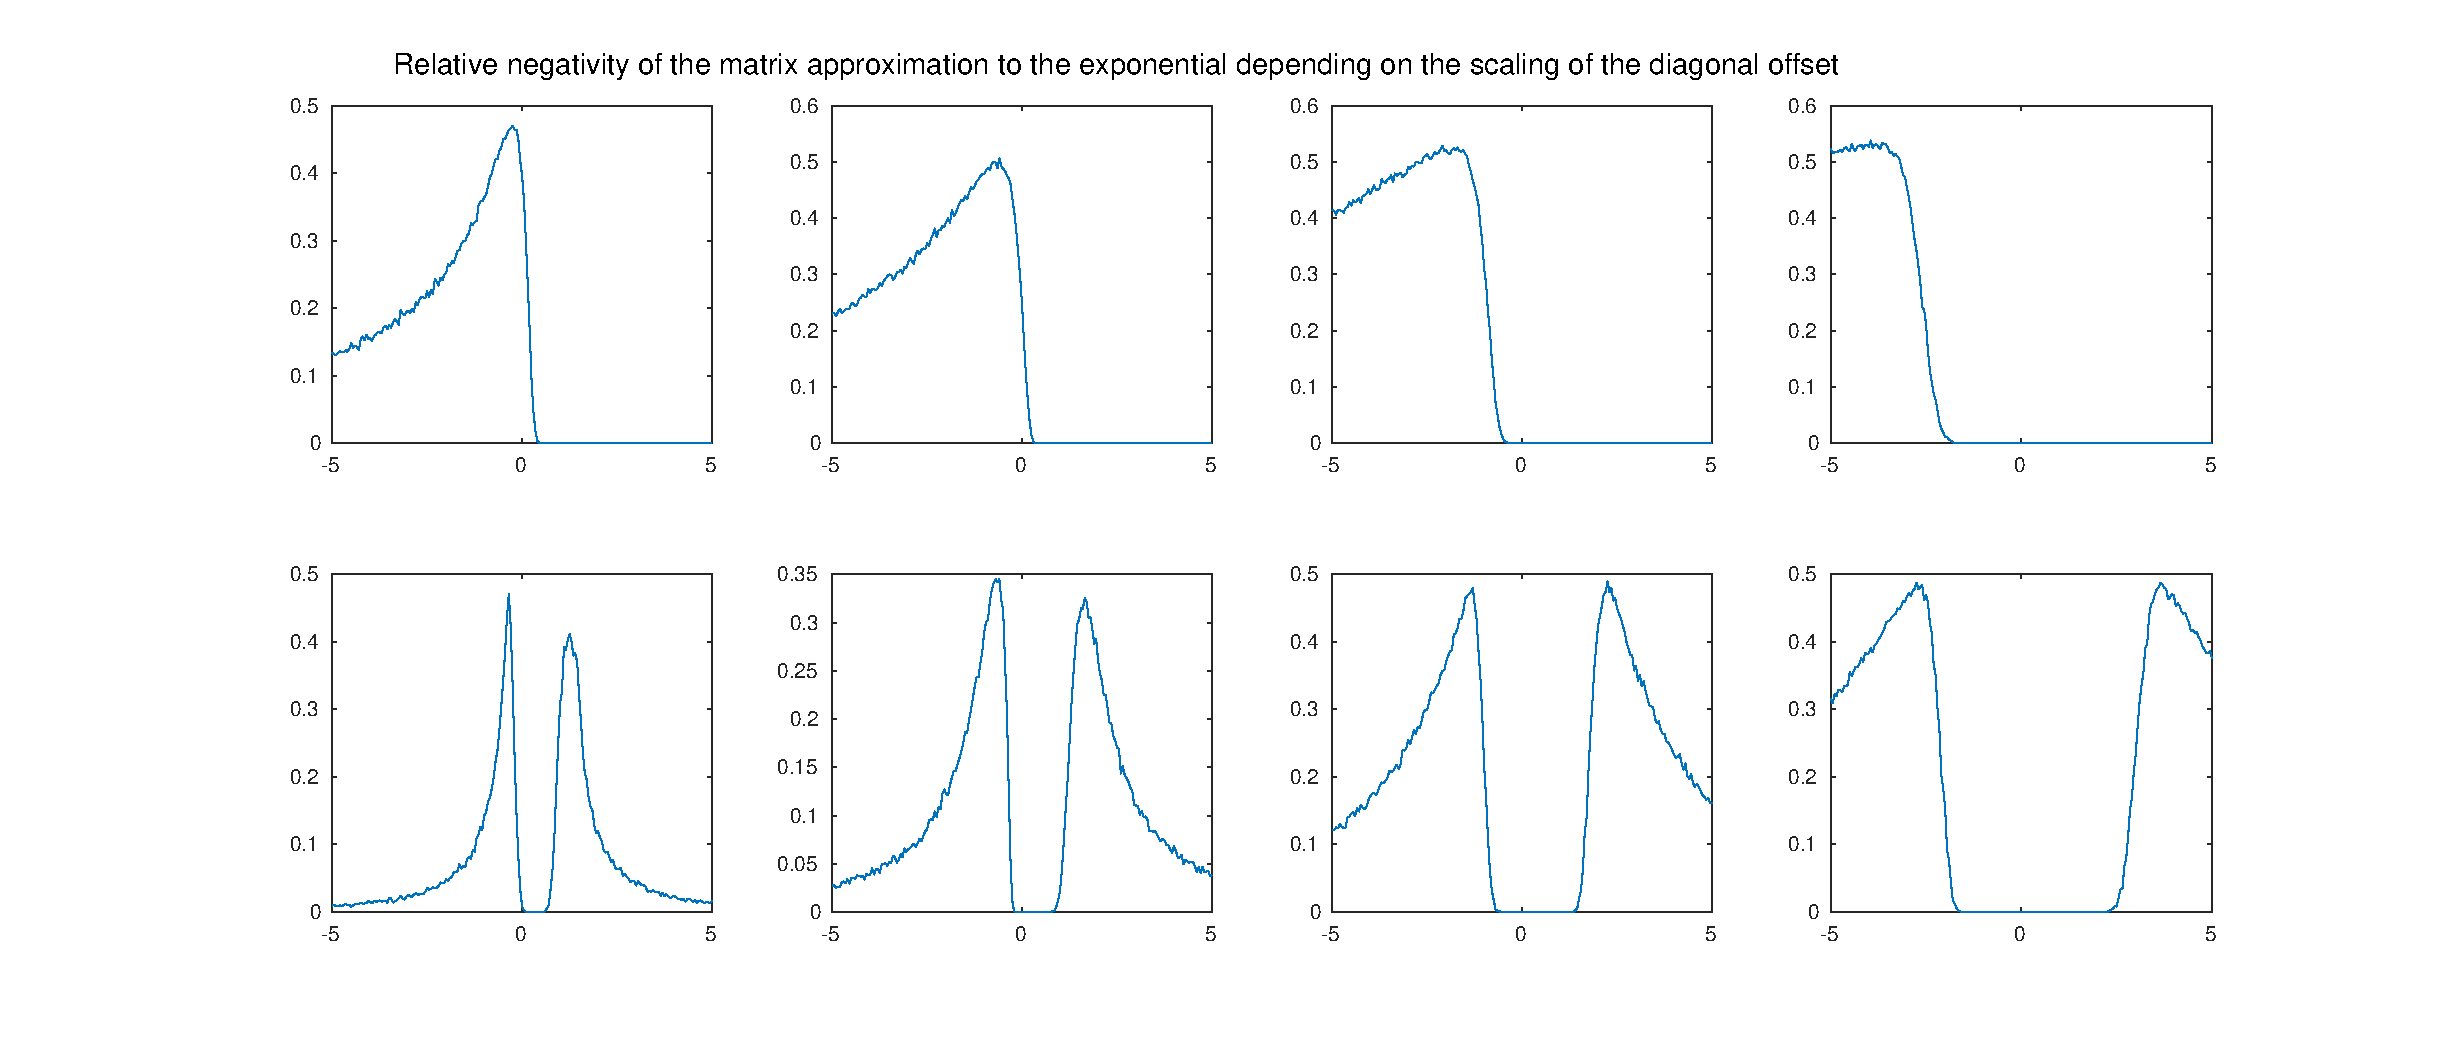
\includegraphics[width=\linewidth]{Matlab/padevsseriesneg.eps}
    \caption{
        Results exploring relative negativity of the approximation of the matrix exponential, as in Figure \ref{fig:padeserieserr}.
        Top row: approximation using the series definition of the matrix exponential.
        Bottom row: approximation using the Pad\'e method.
        The orders of approximations used are not the same as the previous figure, since we stick to diagonal Pad\'e approximations.
        Column 1: second order (Pad\'e $[1,1]$) approximations.
        Column 2: fourth order (Pad\'e $[2,2]$) approximations.
        Column 3: tenth order (Pad\'e $[5,5]$) approximations.
        Column 4: twentieth order (Pad\'e $[10,10]$) approximations.
        The diagonal Pad\'e methods maintain stability for large offset.
    }
    \label{fig:padeseriesneg}
\end{figure}

\begin{figure}
    \centering
    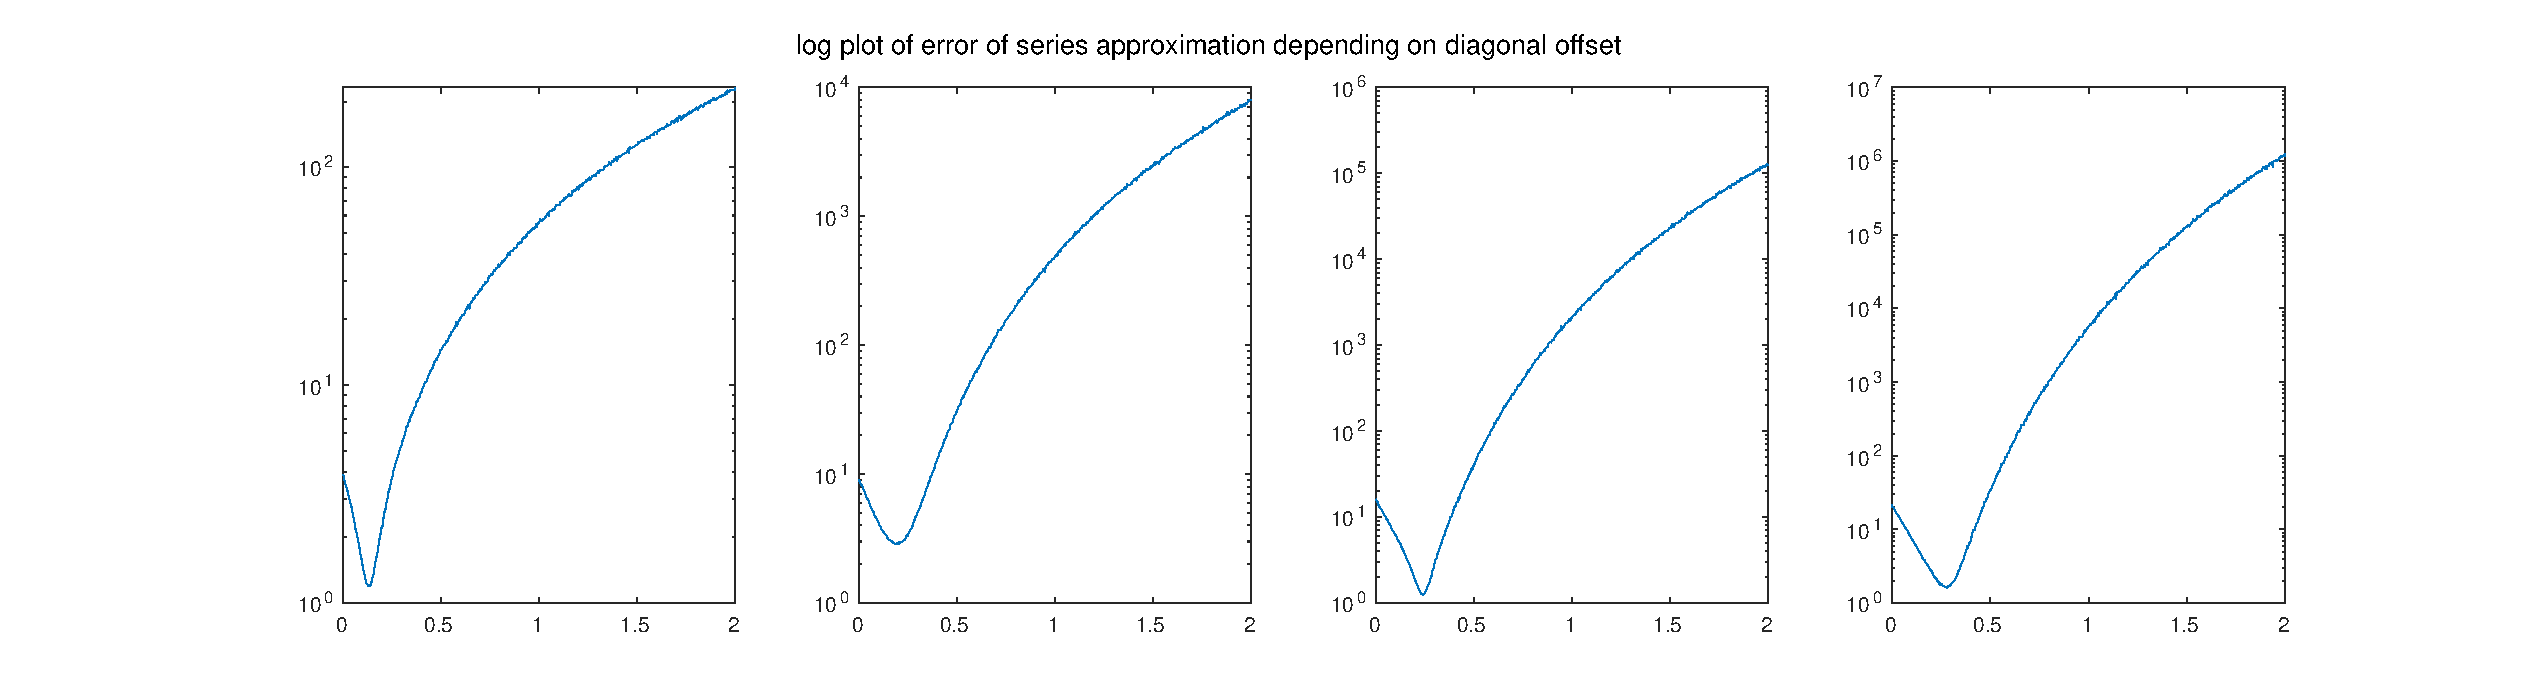
\includegraphics[width=\linewidth]{Matlab/seriesexpminimiser.eps}
    \caption{
        Further visualisation of the error of the series approximation to the product of matrix exponential and vector.
        Logarithmic vertical axis is used for clarity.
        From left to right: error of the approximation of orders $1$ to $4$.
        Using the decomposition $A = \bar{A} + \hat{a}I$, where $\hat{a}= -s |\max(a_{ii})|$, we approximate the matrix exponential using a separation.
        There is clearly always a minimiser over $s$ depending on the order of the method used which gives the best convergence.
        Again using a Monte Carlo estimator for $10 \times 10$ random systems
    }
    \label{fig:serieslog}
\end{figure}

% I think this figure is useless, fig:seriesorder shows enough of it being an approximation
% \begin{figure}
%     \centering
%     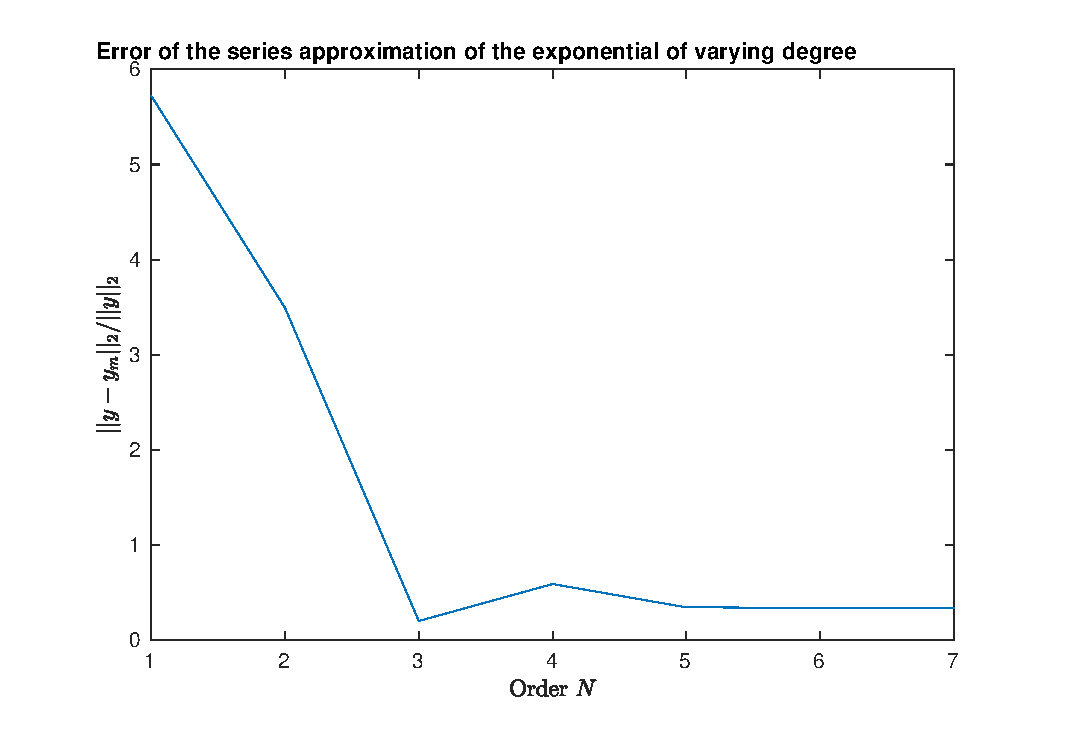
\includegraphics[width=0.75\linewidth]{Matlab/serieserrorwithn.eps}
%     \caption{
%         Visualisation of the convergence of the approximation of the matrix exponential from the series definition using a Monte-Carlo estimate with $500$ samples of random $10 \times 10$ systems.
%         We compute the relative error of the actual product $y = \exp(A)x$ and $y_m = X(A)x$ where $X$ is an approximation using the series up to the term of power $N$.
%         The diagonal offset used was $s=0.4$, which appears to be an approximate minimiser for low order approximations using the series, as shown in Figure \ref{fig:serieslog}
%     }
%     \label{fig:seriesisnotgood}
% \end{figure}

\begin{figure}
    \centering
    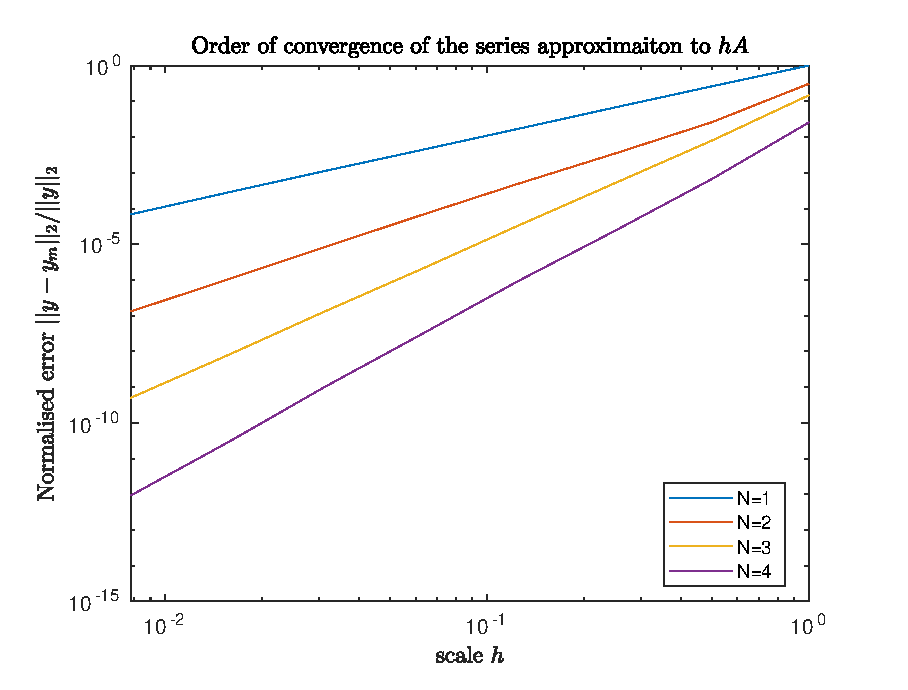
\includegraphics[width=0.65\linewidth]{Matlab/seriesworse.eps}
    \caption{
        Order of convergence of the series approximations of $\exp(hA)x$ depending on $h$, tested on samples of random $4 \times 4$ systems.
        The diagonal offset used was $s = 0.5$, which as shown in Figure \ref{fig:serieslog} appears to be close to a minimiser for low order approximations.
    }
    \label{fig:seriesorder}
\end{figure}

\begin{figure}
    \centering
    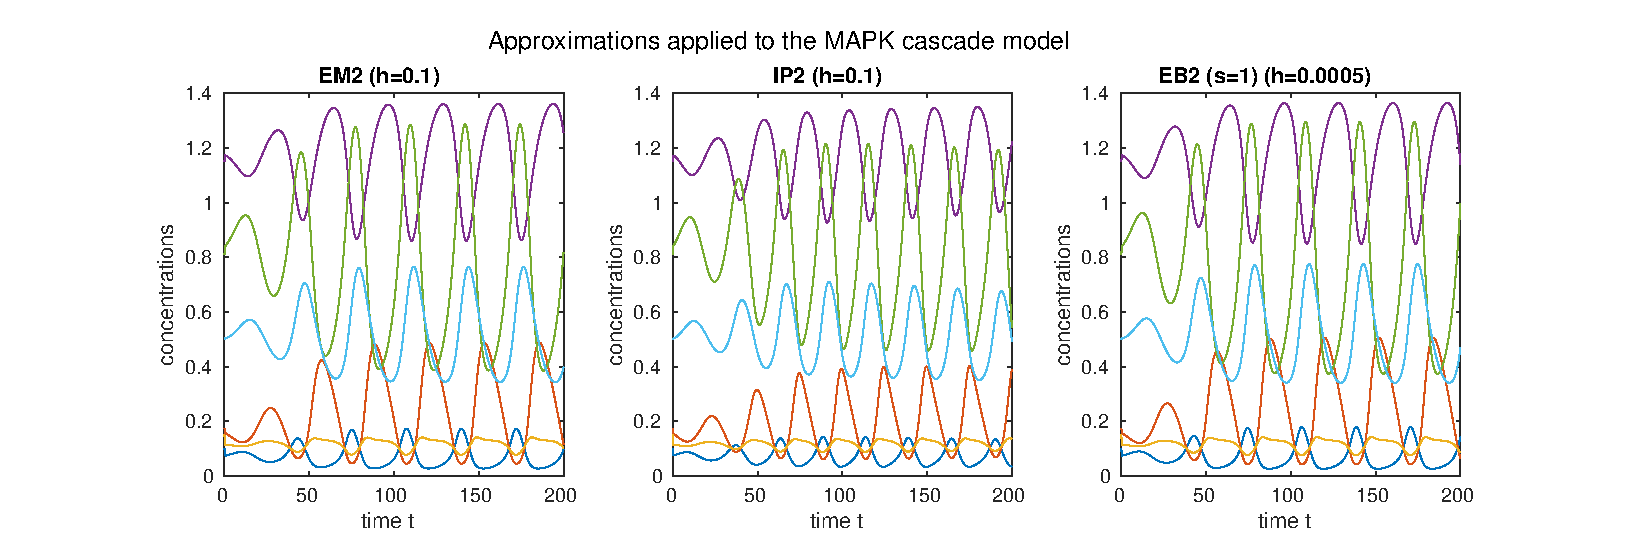
\includegraphics[width=\linewidth]{Matlab/magnustriplemapk.eps}
    \caption{
        Visualisation of the second order Magnus integration when different approximations to the matrix exponential are used.
        Left: EM2, using two matrix exponentials with \texttt{expm()}.
        Middle: IP2, using a first order positivity preserving approximation and a second order Pad\'e.
        Right: EB2, using first and second order approximations to the exponential from the series definition.
    }
    \label{fig:triplemagnus}
\end{figure}

\begin{figure}
    \centering
    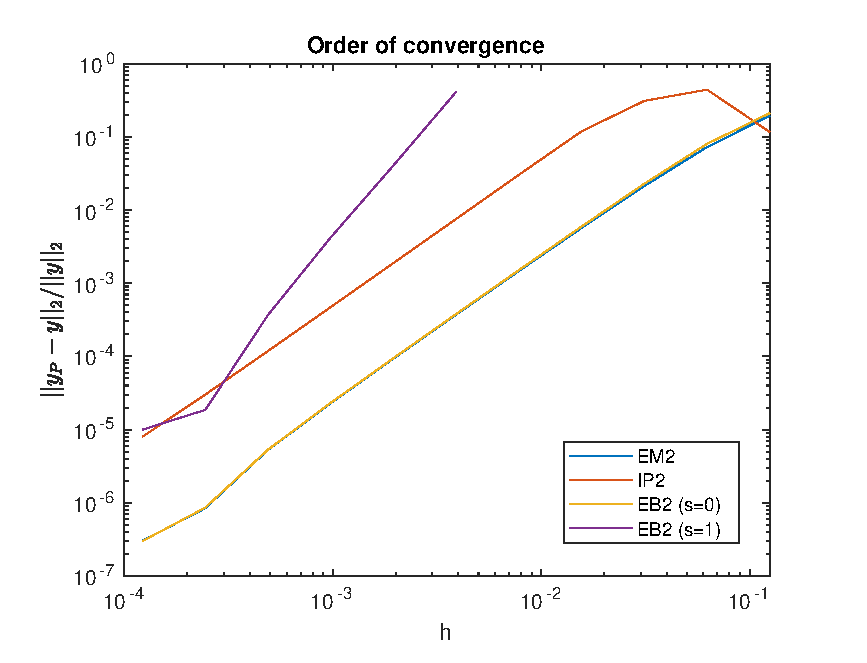
\includegraphics[width=0.65\linewidth]{Matlab/magnusapproximations2.eps}
    \caption{
        Order of convergence for EM2, IP2 and EB2 integration methods.
        We plot the relative error of the solution at end time $T$ against the step size $h$ used in the integration scheme.
        The EM2 method is second order accurate \cite{blanes_pos_2022},
        and IP2 is also second order since their gradients match.
        EB2 is tested for both $s=0$ and $s=1$, but is only theoretically positivity preserving for $s=1$.
    }
    \label{fig:magnusapprxorder}
\end{figure}

In this subsection and the next, we develop our own ideas from those provided by the authors in \cite{blanes_pos_2022},
aiming to use approximations to aid the computational cost of these numerical methods.
We propose an approximation which can be used in the context of positivity preservation.
Theoretically, the approximations should be flexible and positivity preserving.
We will investigate the properties of using the series definition of the exponential, while also considering the priority of positivity preservation.
First, recall for a graph-Laplacian matrix $A$ the reduction $A = \bar{A} + \hat{a}I$ such that $\bar{A}$ is nonnegative.
Therefore $\exp(A) = \exp(\bar{A} + \hat{a}I) = \exp(\hat{a})\exp(\bar{A})$.
In the general case, distribution of the matrix exponential involves the commutator \cite{higham2008exponential},
however the identity matrix commutes with any other square matrix of the same size.

Then, we approximate this matrix exponential using the series definition
\begin{equation*}
    \exp(\bar{A}) \approx \sum_{k=0}^{N} \frac{1}{k!}A^k =: T_N(\bar{A}).
\end{equation*}
Clearly $T_N$ is an $N$-th order approximation to the matrix exponential.
Therefore
\begin{equation*}
    \exp(A) = \exp(\hat{a})T_N(\bar{A}) + \mathcal{O}(h^{N+1}).
\end{equation*}
However, we apply the approximation to both the matrix and the scalar exponentials, so our approximation takes the form
\begin{equation}
    \exp(A) = T_N(\hat{a})T_N(\bar{A}) + \mathcal{O}(h^{N+1}).
\end{equation}
Furthermore, since $\bar{A}$ is entirely positive, we would expect the approximation to be positivity preserving.
We acknowledge that we have given notable attention earlier to the impracticality of using the series expansion on its own, and now we are using the series expansion in our approximation.
We will return to this point later.
See Figures \ref{fig:padeserieserr} and \ref{fig:padeseriesneg}, evaluating the behaviour of approximations to the matrix exponential and vector product.
As we mentioned earlier, the computation of the matrix exponential by a series expansion can be very unstable,
which we observe here.
This brings attention to the first problem with this approach: the series approximation by itself is fairly poor for low order approximations, compared to Pad\'e. % more on this?
% See also Figure \ref{fig:seriesisnotgood}, which illustrates the remainders left when using order $N$ approximations to the matrix exponential.
% The order N approximation of hA should converge if norm(hA) < 1 (strictly is useful)

Consider the example given at the beginning of the discussion of the Pad\'e approximation.
We have the matrix
\begin{equation*}
    A = \begin{bmatrix}
        -4 & 1 & 0 \\
        2 & -1 & 2 \\
        2 & 0 & -2
    \end{bmatrix}
\end{equation*}
and vector
\begin{equation*}
    x = \begin{bmatrix}
        3 \\
        1 \\
        2
    \end{bmatrix}.
\end{equation*}
We evaluate $y = \exp(A)x$ in MATLAB using \texttt{expm()} and provide an approximation $y_m = T_N(\hat{a})T_N(\bar{A})x$ given the required order $N$.
We have visualised this approximation in Figure \ref{fig:serieslog}, where we can identify positions of optimality for the approximations depending on $s$.
The minimum region of values for $s$ required for optimal error is always strictly less than $1$.
Note that this leads to another problem: in order for the method to preserve positivity in theory, we require $s \ge 1$, however the optimal values of $s$ for our lower order approximations do not satisfy this constraint.
Despite this, we continue. 
Instead of comparing the convergence of different order approximations to the matrix exponential,
it may be insightful to apply these methods to an integrator and compare with the methods and approximations have already been established.

Note the results given in Figure \ref{fig:seriesorder}. The convergence of these methods follow steeper gradients as $N$ increases as the remainder in $\mathcal{O}(h^N)$ decreases.
This figure generates a random graph-Laplacian matrix $A$ and random vector $x$, and then evaluates a relative error $||y-y_N||_2/||y||_2$,
where $y = \exp(A)x$ and $y_N = T_N(A)x$.
We can deduce that the error should be $\mathcal{O}(||A||^{N+1})$ for some subordinate matrix norm on $A$.
Figure \ref{fig:seriesorder} also uses a value of the scaling parameter $s$ which we recognise does not guarantee positivity preservation,
instead it has been chosen to improve the approximation in a sense of relative error.
This demonstrates a third problem with using the series approximation: the approximation is unlikely to converge for low order $N$,
and the norm of the matrix plays a large role in the error of the approximation.
Increasing the scaling parameter $s$ means we are taking the exponential of a matrix with a larger diagonal, and hence with a larger spectral norm.
Therefore if we increase $s$ to ensure positivity, our approximation will be, in a sense of relative error, worse.

We will now evaluate an experiment, considering how we can apply approximations to the matrix exponential to numerical methods.
We will consider three methods, all of which are variations of the EM2 Magnus integrator, using
\begin{itemize}
    \item EM2: Two matrix exponentials, computed using \texttt{expm()}.
    \item IP2: One first order approximation using $[I-hA]^{-1}$ and one second order diagonal Pad\'e approximation.
    \item EB2: One first order and one second order approximation using the series method proposed, with scaling parameter chosen to consider positivity preservation. 
\end{itemize}
We will examine each of these methods applied to the MAPK cascade.

For IP2, we used the reduction $A = \bar{A} + \hat{a}I$ with $a = -s |\max(a_{ii})|$ and chose $s=1$ to adhere to the method outlined by \cite{blanes_pos_2022},
namely that this should be positivity preserving. In our discussion on the Pad\'e approximation we showed why positivity is not necessarily preserved.
For the EB2 method, we used first and second order series approximations with both $s=0$ and $s=1$.
From our testing, $s=0$ meant the approximation was more usable but not unconditionally positivity preserving.
We found that increasing $s$ makes the computation of EB2 far more expensive, and unusable for moderate $h$.
It would not be useful to consider negative values of $s$ since we have discussed that this is not appropriate for positivity preservation.
% s=0 for series and pade s=1 
First, see Figure \ref{fig:triplemagnus}. We show the behaviour of the integration from EM2, IP2 and EB2 on separate figures.
The EM2 and IP2 integrations appear similar, which follows from the results concluded by \cite{blanes_pos_2022},
being that the EM2 method is second order accurate.
Furthermore, the IP2 method retains the second order accuracy of EM2, since it uses a positivity-preserving first-order approximation, followed by a second order Pad\'e approximation. 
It is important to recall that we have shown that this Pad\'e approximation is not positivity preserving.
The EB2 method, using series exponentials, is surprisingly accurate to EM2.

Finally, observe Figure \ref{fig:magnusapprxorder}, where we show the convergences of the methods.
To compute the order of convergence of these methods, we obtain a solution to the problem using \texttt{ode45()} with an extremely low error tolerance,
which we refer to as the master solution.
We integrate the system up to time $T=200$ and store the final value.
Then, given a value of $h$, we integrate the system again using a positivity preserving method.
We repeat this for a range of values of $h$ decreasing in magnitude in order to plot the rate of convergence.
We use the vector $2$-norm to obtain a relative error given by $||y_P - y||_2 / ||y||_2$,
where $y$ is our master solution and $y_P$ is our approximation.
This provides sufficient data to visualise the order of convergence of a numerical method of our choice.
We repeat this for all the methods we wish to analyse.

Since EM2 and IP2 are both second order, they converge to the ``exact'' solution at the same rates.
We have graphed EB2 choosing both $s=0$ and $s=1$. For $s=0$, the approximation is not guaranteed to preserve positivity,
but the approximation follows the order of EM2 closer than the IP2 approximation.
Choosing $s=1$ means we are approximating the exponential in a way that guarantees positivity.
However, the approximation becomes prohibitively expensive, and IP2 is a better method for timesteps $h > 10^{-3}$.
In fact, for timesteps $h > 10^{-2}$ the error of the approximation is so large that the method is unusable - the error is outside the visible region of the graph. 
For extremely small timesteps $h \approx 10^{-4}$ EB2 is only ever as good as IP2.
Essentially, the error between EM2 and EB2 is that we can save on computing matrix exponentials with EB2,
but we may need to perform a thousand timesteps in the place of one.

The main problem with EB2 is that when we apply the reduction $A = \bar{A} + \hat{a}I$ and start working with the diagonal offset parameter $s$,
we want $s \ge 1$ in order to guarantee positivity, but optimal error is attained out of this bound (recall Figure \ref{fig:serieslog}).
This problem gets worse when we look at how the diagonal offset affects $\bar{A}$, because if $s$ is sufficiently large then it scales with the spectral radius of $\bar{A}$,
and taking a low order sereis approximation of the exponential of this matrix is going to be less accurate as this increases.
In simpler terms, by using the series approximation and being given control of the diagonal offset, it is challenging to have both positivity and convergence.

% And then if we forget about error and just focus on positivity, enforcing $s > 1$ brings about a third problem: if $s$ is sufficiently large,
% then we are increasing the norm %WHAT NORM
% of the matrix we are approximating,
% and taking a low order approximation of the exponential, from the series definition, of this matrix is going to diverge as this norm increases.
% In simpler terms, by using the series approximation and being given control of the diagonal offset, having both positivity and convergence is impossible.

% The EB2 method, however, appears to not converge at all. Any change in the relative error is not even visible on the graph since it appears as a flat line.
% This is likely because refining the timestep does not change how the method appears to solve the problem on a slower timescale - the solution will refine but it will still be fundamentally incorrect in terms of time.
% It would be interesting to explore the behaviour of EB2 if we were able to manipulate the parameters to improve accuracy,
% perhaps by optimising the method using a different diagonal offset scaling $s$, and slightly higher degree approximations to the matrix exponential.

%% To review the proposed method once it has been completely covered
% first introduce the series approximation and the guarantee of positivity under certain values of s
% problem 1: series definition is not as good as pade and provides poor approximations
% problem 2: optimal value of s is not in the bound s >= 1
% problem 3: large values of s theoretically guarantees positivity, however this increases the norm of the matrix which makes the series even more unusable
% "by using the series approximation with diagonal offset, having both positivity and convergence is impossible"

\subsection{A Proposed Improvement to the Pad\'e Approximation}

\begin{figure}
    \centering
    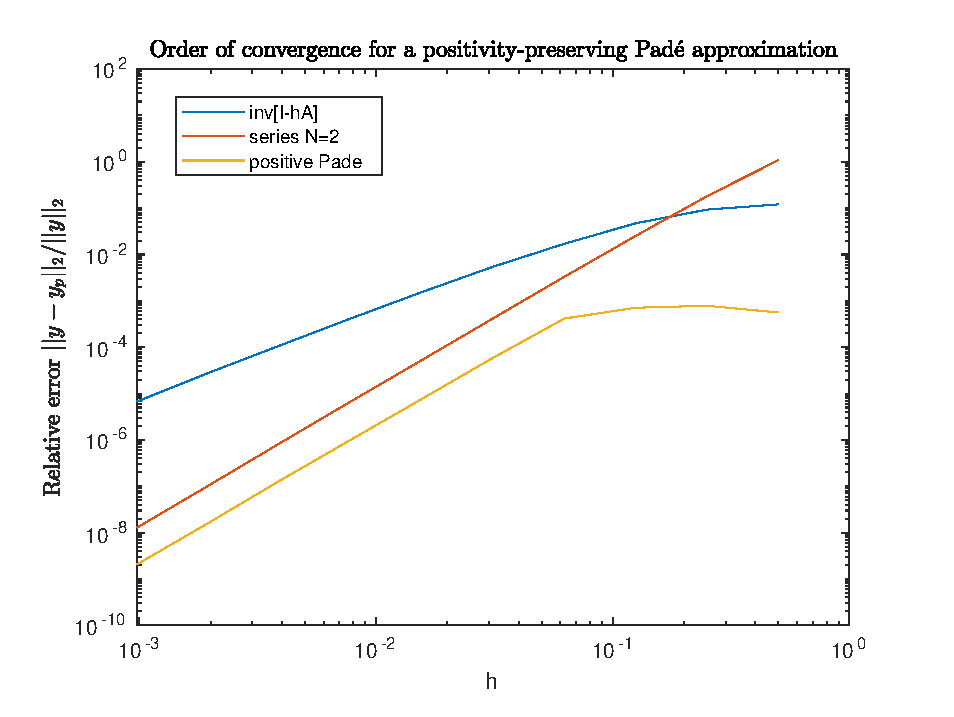
\includegraphics[width=0.75\linewidth]{Matlab/positivepadeconvergence.eps}
    \caption{
        Order of convergence for the positivity preserving modification to the $[1,1]$ Pad\'e approximation to the matrix exponential.
        The order matches a given second order approximation.
        The construction of this approximation guarantees positivity.
    }
    \label{fig:padepositive}
\end{figure}

\begin{figure}
    \centering
    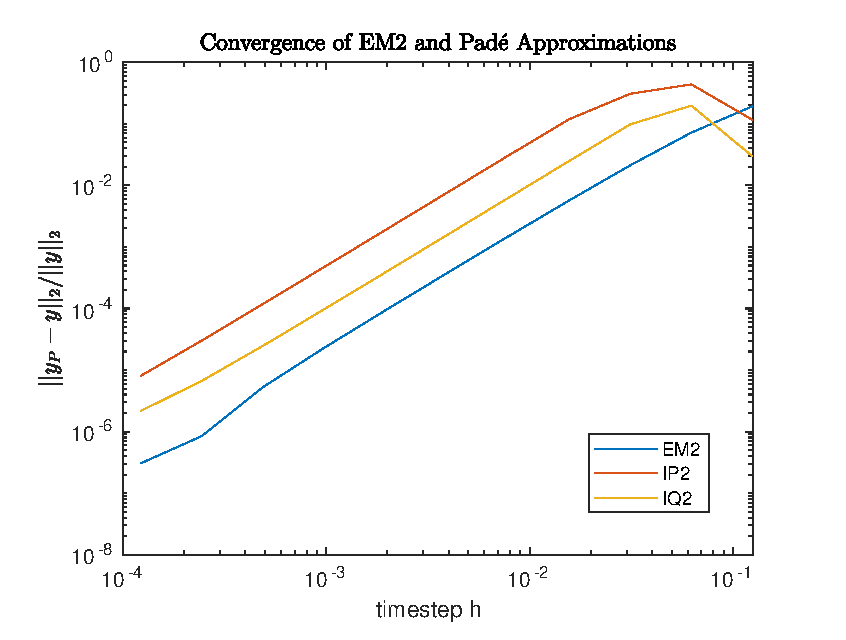
\includegraphics[width=0.75\linewidth]{Matlab/positivemapk2.eps}
    \caption{
        Methods EM2, IP2 and IQ2 applied to the MAPK problem, evaluating the global error as a function of the timestep.
        All methods are clearly second order, however EM2 uses directly computed matrix exponentials from \texttt{expm()},
        while IQ2 uses positivity-preserving approximations.
        IP2 is as we have defined earlier.
        EM2 solution computed in 196.7 seconds.
        IP2 solution computed in 324.5 seconds.
        IQ2 solution computed in 346.0 seconds.
    }
    \label{fig:pademapkpos}
\end{figure}

Developing from before, we will consider using more robust techniques to again improve the cost of a numerical integration scheme from \cite{blanes_pos_2022}.
The following method applies many results that we have explored in this section.
First, the construction of the Pad\'e approximation.
Second, the implementation of scaling and squaring.
Third, the decomposition $A = \bar{A} + a I$
Third, Lemma \ref{lem:positiveinverse} on the positivity of the inverse $[I - A]^{-1}$.

We propose a numerical integration scheme which is another modification of EM2, except using two matrix exponential approximations which are positivity preserving.
This method is identical to the IP2 method we introduced in the previous section, except for the modification of the second order Pad\'e approximation.
Hence this is the change that we will discuss here.

%TODO: come back here
Recall Lemma \ref{lem:positiveinverse} - clearly scaling is useful.
Then using the Pad\'e approximation,
\begin{align*}
    \mathrm{e}^{hA} &= \left[ \mathrm{e}^\frac{hA}{2^m} \right]^{2^m} \\
    &= \left[
        \left[ I - \frac{hA}{2^{m+1}} \right]^{-1} \left[ I + \frac{hA}{2^{m+1}} \right] + \mathcal{O}(h^2)
    \right]^{2^m} \\
    &= \left[
        \left[ I - \frac{hA}{2^{m+1}} \right]^{-1} \left[ I + \frac{hA}{2^{m+1}} \right]
    \right]^{2^m} + \mathcal{O}(h^2) \\
\end{align*} 
so clearly this is a valid approximation method.

Our approximation method is as follows.
First, we deconstruct $A$ as per $A = \bar{A} + \hat{a}I$, as we have looked into earlier.
We ignore any scaling parameter in this choice, implicitly taking $s=1$ by having $\hat{a}$ being the most negative entry on the diagonal of $A$.
We can then approximate the exponential by taking $\exp(A) = \exp(a)\exp(\bar{A})$ and approximating the exponential of $\bar{A}$.
We can choose to approximate the scalar or compute it directly, as computing the scalar exponential is not considered computationally expensive - we have found there is not a significant error in either case.
For the Pad\'e $[1,1]$ approximation of $\bar{A}$, we can guarantee the numerator matrix will be positive regardless of its scaling.
In order to ensure positivity of the denominator matrix, we find a scaling $2^m$ such that $\bar{A}/2^m$ satisfies the bound required in Lemma \ref{lem:positiveinverse}.
There is a trick here. In order to satisfy the bound, we need to know the $2$-norm of $\bar{A}$.
However, we know that $||A||_2 < \sqrt{d}||A||_1$ in general \cite{horn2012matrix}, where $d$ is the dimension of the matrix.
The $1$ norm is the maximum column sum of the matrix. However, since $A$ is a graph-Laplacian matrix, the maximum column sum of $\bar{A}$ is $\hat{a}$ by construction.
Hence we don't need to make any computations on the properties on the matrix.
We compute the Pad\'e approximation for the scaled-down matrix, then repeatedly square to return to the original scale.
This gives us a $[1,1]$ Pad\'e approximation which guarantees positivity.

This is a simplified version of the actual method implemented by MATLAB to compute the matrix exponential.
Cost is reduced by computing the $[1,1]$ approximation,
and by not needing to compute any matrix norms.

We have shown the results of this implementation in Figures \ref{fig:padepositive} and \ref{fig:pademapkpos}.
The former indicates that the matrix approximation is itself second order accurate,
while the latter indicates that EM2 maintains second order accuracy when this approximation is implemented.
Rate of convergence is computed again by comparing the final values of the solution to that of a master solution, obtained using \texttt{ode45()} method with extremely low tolerance,
and computing a relative error in the $2$-norm.
We can see that IQ2 retains second order accuracy.
The IQ2 method is unconditionally positivity preserving, unlike the IP2 method proposed by the authors in \cite{blanes_pos_2022}, as we have explored earlier.
Furthermore, we can see from Figure \ref{pademapkpos} that the IQ2 method provides a closer approximation than IP2.

Note that in Figure \ref{fig:pademapkpos} we have stated the computation times of both methods for solving the IVP.
Despite our implementation taking longer than the internal function,
this is expected since the core included functions for MATLAB run using compiled FORTRAN code which is much faster in general than the interpreter for MATLAB itself \cite{moler2020history}.

Implementation of our positivity preserving Pad\'e approximation in integration schemes is given in Appendix \ref{apn:exp}.

\section{Wider Positivity Preservation}

\subsection{The Implicit Euler Method}
% backward Euler
% unconditionally positivity preserving methods are stuck at first order
Consider a system defined in its most general form by $\dot{x} = f(t,x)$.
Let $y$ be the solution to the backward Euler method, so given $x = x_n$ we require $y = x_{n+1}$ to satisfy.
\begin{equation*}
    y = x + h f(t,y)
\end{equation*}
The following result shows that this method is positivity preserving.
\begin{theorem}[Hundsdorfer, Verwer (2003) \cite{hundsdorfer2003numerical}]
    The implicit Euler method is unconditionally positivity preserving for any positive step size $h > 0$.
\end{theorem}
\begin{proof}
    The expression for the method is $y = x + hf(t,y)$, which we assume is continuous depending on $h$, where $t$ and $x$ are fixed.
    This does require the continuity of $f$.
    We write this method as a function $y(h)$, where the result depends on a parameter $h$ for fixed $t$ and $x$..
    Our aim is to show that if $x$ is nonnegative then so is $y(h)$ for all $h$, however it is sufficient to prove this for a given $h$.
    This is because $y$ is continuous on $h$, and $h$ is chosen arbitrarily, so $y$ will stay within the positive region.
    Assume that, given some positive $h_0$, we have that $y(h) > 0$ for $h < h_0$, except for the $i$-th entry where we assume $y_i(h_0) = 0$.
    Then we have
    \begin{equation*}
        0 = y_i(h_0) = x_i + h_0 f_i(t, y(h_0)).
    \end{equation*}
    The coefficient $h_0$ is positive, and we assumed $v_i$ is nonnegative. In order for the problem to preserve positivity we require that $f_i(t, y(h_0))$ be nonnegative.
    In the case that $x_i = 0$ and the same for $f_i$, then $y_i = 0$ so the $i$-th entry in the solution remains at zero.
    Otherwise, we have a contradiction, meaning that if $x$ is positive then the implicit Euler method preserves positivity.
\end{proof}
The proof, as given in the textbook \cite{hundsdorfer2003numerical}, causes some confusion with the implementation of the implicit Euler method at a fixed $t$.
If it was instead given for some evaluation of $f(t,y(h))$ where $t = t_0 + h$, the process would be more clear since we are clearly computing $f$ at the time $t_{n+1}$ and value $y = x_{n+1}$ of the solution.

The result lends some similarity to when we discussed positivity preservation of a problem governed by a graph-Laplacian matrix in Theorem \ref{thm:posgl}.
The assumption of the behaviour of the derivative at zero is key to the result, since this is the behaviour that preserves positivity.
When discussing earlier in this chapter, we used the result in a linear case, but have now been able to show it generally.
Interestingly, the connection between these two results is even more evident when we consider how this does in fact apply to problems of the form $\dot{x} = A(x)x$,
where $A$ is a graph-Laplacian matrix.
The implicit Euler method applied to this problem is 
\begin{equation*}
    x_{n+1} = x_n + h A(x_{n+1})x_{n+1}
\end{equation*}
which rearranges to
\begin{equation*}
    x_{n+1} = \left[
        I - h A(x_{n+1})
    \right]^{-1}x_n
\end{equation*}
which we know is positivity preserving.
The positivity preservation of this matrix can be seen as another case of this general result on the behaviour of the backward Euler method.

It is widely recognised that there are no methods which, when applied to generally formulated problems, preserve positivity unconditionally and also have truncation error of order greater than $1$.
This result is stated in \cite{bolley1978conservation}, and referenced in \cite{blanes_pos_2022, hundsdorfer2003numerical} and others. 

\subsection{Review}

We have given an overview on current methods in positivity preservation.
The focus of our analysis has been the formulation and improvement of second-order methods.
This contrasts to symplectic and more general geometric integrators,
where we have fourth and higher order schemes available.
In a sense, this is one limitation of the analysis we have provided,
namely that we have studied improvements over current methods,
but have not provided any framework for how we would formulate higher-than-second-order methods.
This itself is still an active area of research.

Having finished our analysis of positivity preservation, we provide a discussion to review all the topics from this report.
